\chapter{Distributed System}
\section{Communication}
There are two type of communication character:
\begin{itemize}
    \item \textbf{Communication entities:} can answer the question \textit{"What is Communication?"}
    \item \textbf{Communication paradigm:} concerns on \textit{"How do they communicate?"}
\end{itemize}
\textbf{Entities} can be called as:
\begin{itemize}
    \item \textit{Nodes or Processes} $\rightarrow$ \textbf{system-oriented entities}
    \item \textit{Components, objects or web services} $\rightarrow$ \textbf{problem-oriented entities}
\end{itemize}
These entities can communicate using \textbf{different paradigms:}
\begin{itemize}
    \item \textbf{Interprocess communication:} refers to the relatively \textit{low-level support} for communication between processes in distributed systems
    \item \textbf{Remote Invocation:} covers a range of techniques based on a \textit{two-way exchange} between communicating entities in a distributed system and resulting in the calling of a remote operation, procedure or method. In other words, it is based on the idea of \textbf{ask/use methods implemented by a remote process.} Like:
        \begin{itemize}
            \item Request-replay protocols
            \item Remote procedure calls
            \item Remote method invocation
        \end{itemize}
    \item \textbf{Indirect Communication}: allows a strong \textbf{degree of decoupling (disaccoppaimento)} between \textit{senders} and \textit{receivers}. Senders don’t need to know who they are sending to and both senders and receivers don’t need to exist at the same time. Like: 
        \begin{itemize}
            \item Group-communication
            \item Publish-subscribe.
        \end{itemize}
\end{itemize}

\section{Hardware Organization}
The main goal of the hardware organization is to \textbf{improve the performance while maintaining the cost as low as possible.} There can be developed:
\begin{itemize}
    \item \textbf{Centralized System:} that increase the CPU speed but gas some physical constraints
    \item \textbf{Distributed system:} for which there can be different various models divided according to the \textbf{Flynn Classification}:
    \begin{figure}
        \centering
        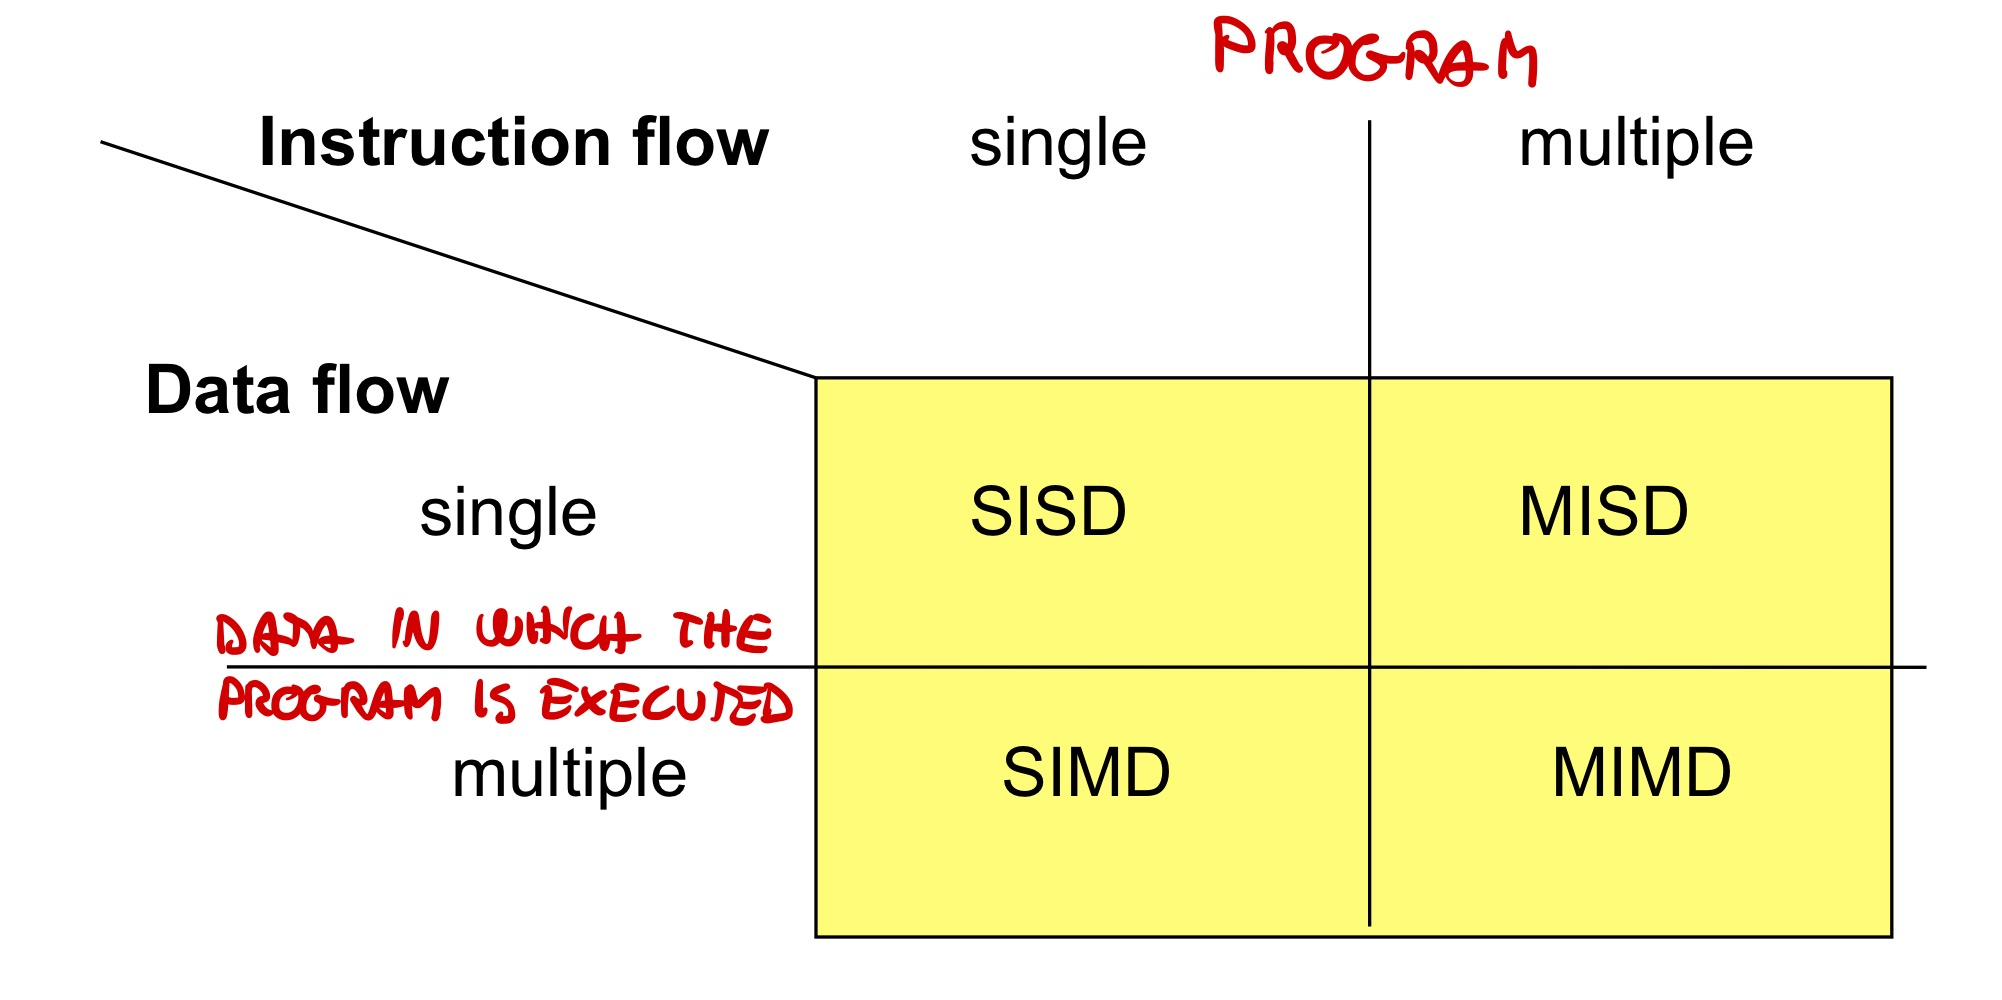
\includegraphics[width=.7\linewidth]{images/distributedSystem/DSArchitecture.jpeg}
        \caption{Flynn Classification}
    \end{figure}
\end{itemize}
Now we analyse each element of the table
\begin{itemize}
    \item \textbf{SISD:} it corresponds to the Von Neumann model with a \textit{single program executed by a CPU and data stored inside the memory.} In order to improve the performance of the system some techniques are adopted like:
        \begin{itemize}
            \item \textbf{Parallelism:} in which are used many specialized ALU that execute each single operation with high speed
            \item \textbf{Pipeling:} in which are executed simultaneously more operations for different instructions
            \item \textbf{Hierarchies of Memory:} like cache levels
            \item \textbf{Specialized Hardware}
        \end{itemize}
    \begin{figure}[!h]
                \centering
                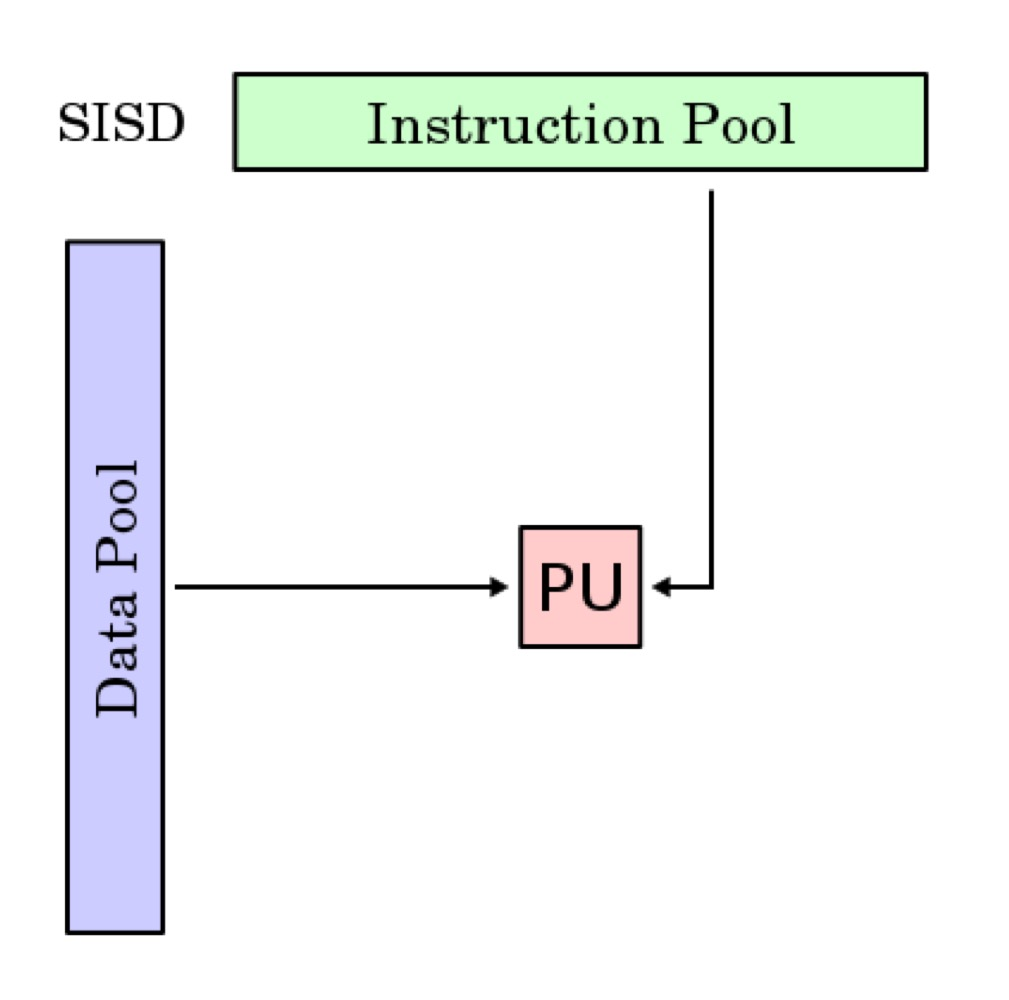
\includegraphics[width=.30\linewidth]{images/distributedSystem/SISD.jpeg}
                \caption{SISD}
            \end{figure}
    \item \textbf{SIMD:} typical of parallel execution in which there’s a \textit{unique program executed on a set of data.} This system is implemented inside a single PC.  Also in this case there can be different architectures that determine how to organise the system, like: 
    \begin{itemize}
        \item \textbf{Vectorial Architecture:} where instead of one ALU that works on a single variable for each input, there is a vector of ALU working on a vector of input values and producing a vector of output.
        \item \textbf{Array Processor:} represented as a matrix processor x memory, in which each processor executes the instruction on the available data in the local storage.
    \end{itemize}
     \begin{figure}[!h]
            \centering
            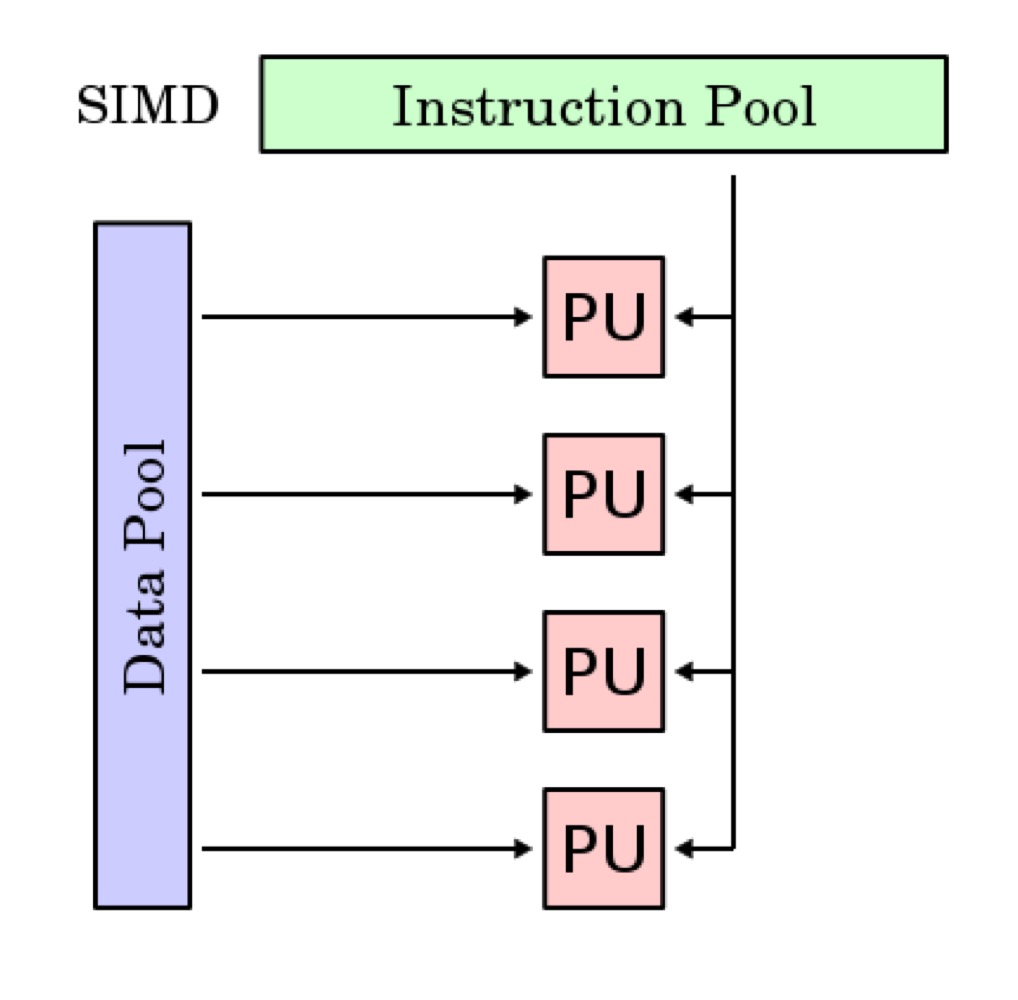
\includegraphics[width=.30\linewidth]{images/distributedSystem/SIMD.jpeg}
            \caption{SIMD}
        \end{figure}
   
    \item \textbf{MISD:} Multiple Instruction Single Data
    \begin{figure}[htp]
            \centering
            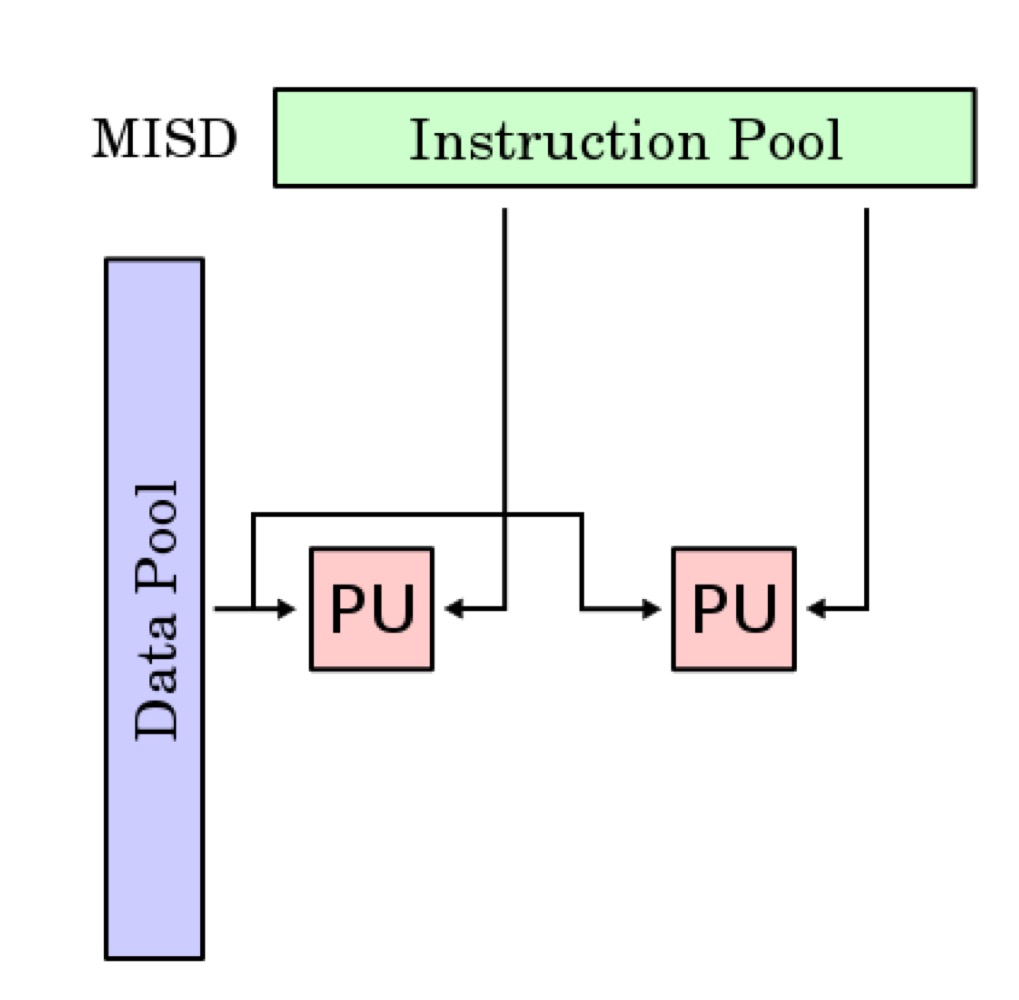
\includegraphics[width=.30\linewidth]{images/distributedSystem/MISD.jpeg}
            \caption{MISD}
        \end{figure}
    
    \item \textbf{MIMD:} typical distributed systems in which \textit{ different CPU executes different programs on different data streams.} Each CPU is associated with his Program Counter, memory, data and programs and they cooperate to execute and provide a common service.
    A MIMD system, implemented by a distributed system, can be organized in different ways, \textbf{\textit{Multiprocessor} or \textit{Multicomputer}}.
    \begin{figure}[htp]
            \centering
            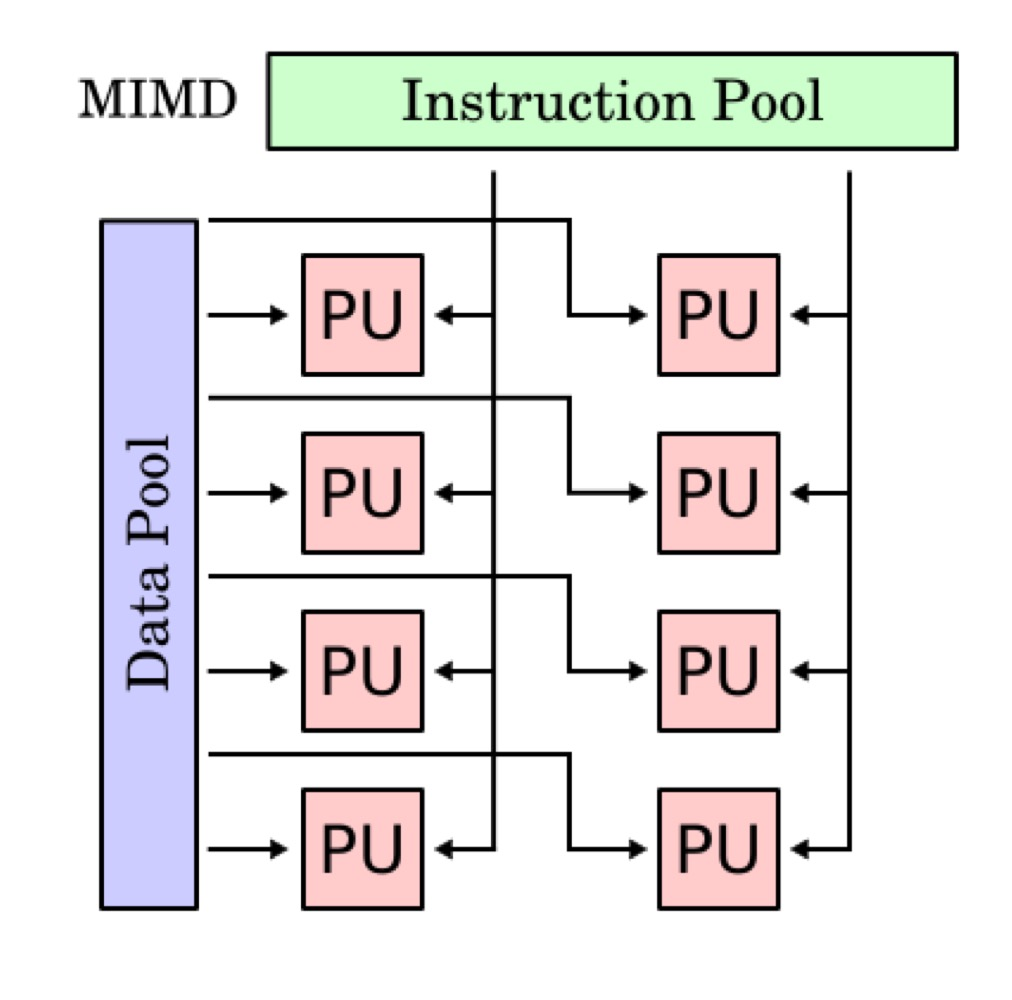
\includegraphics[width=.30\linewidth]{images/distributedSystem/MIMD.jpeg}
            \caption{MIMD}
    \end{figure}
    
\end{itemize}

\newpage
\section{Multiprocessor}
\textbf{Multiprocessor} is characterised by a \textit{set of CPUs} connected in a \textit{communication network} in which there is a \textbf{shared memory.} The advantage of this design, since CPUs are \textbf{strictly coupled}, are that:
\begin{itemize}
    \item It has \textbf{short transmission delay}
    \item And \textbf{high transmission speed}
\end{itemize}

\subsection{Bus}
CPUs are connected in a \textbf{bus} and they \textit{share the same memory.} They have to interact to determine who can access the shared memory. We can imagine that it is necessary to \textbf{implement a synchronisation system  to access the memory.}
\begin{figure}[!h]
            \centering
            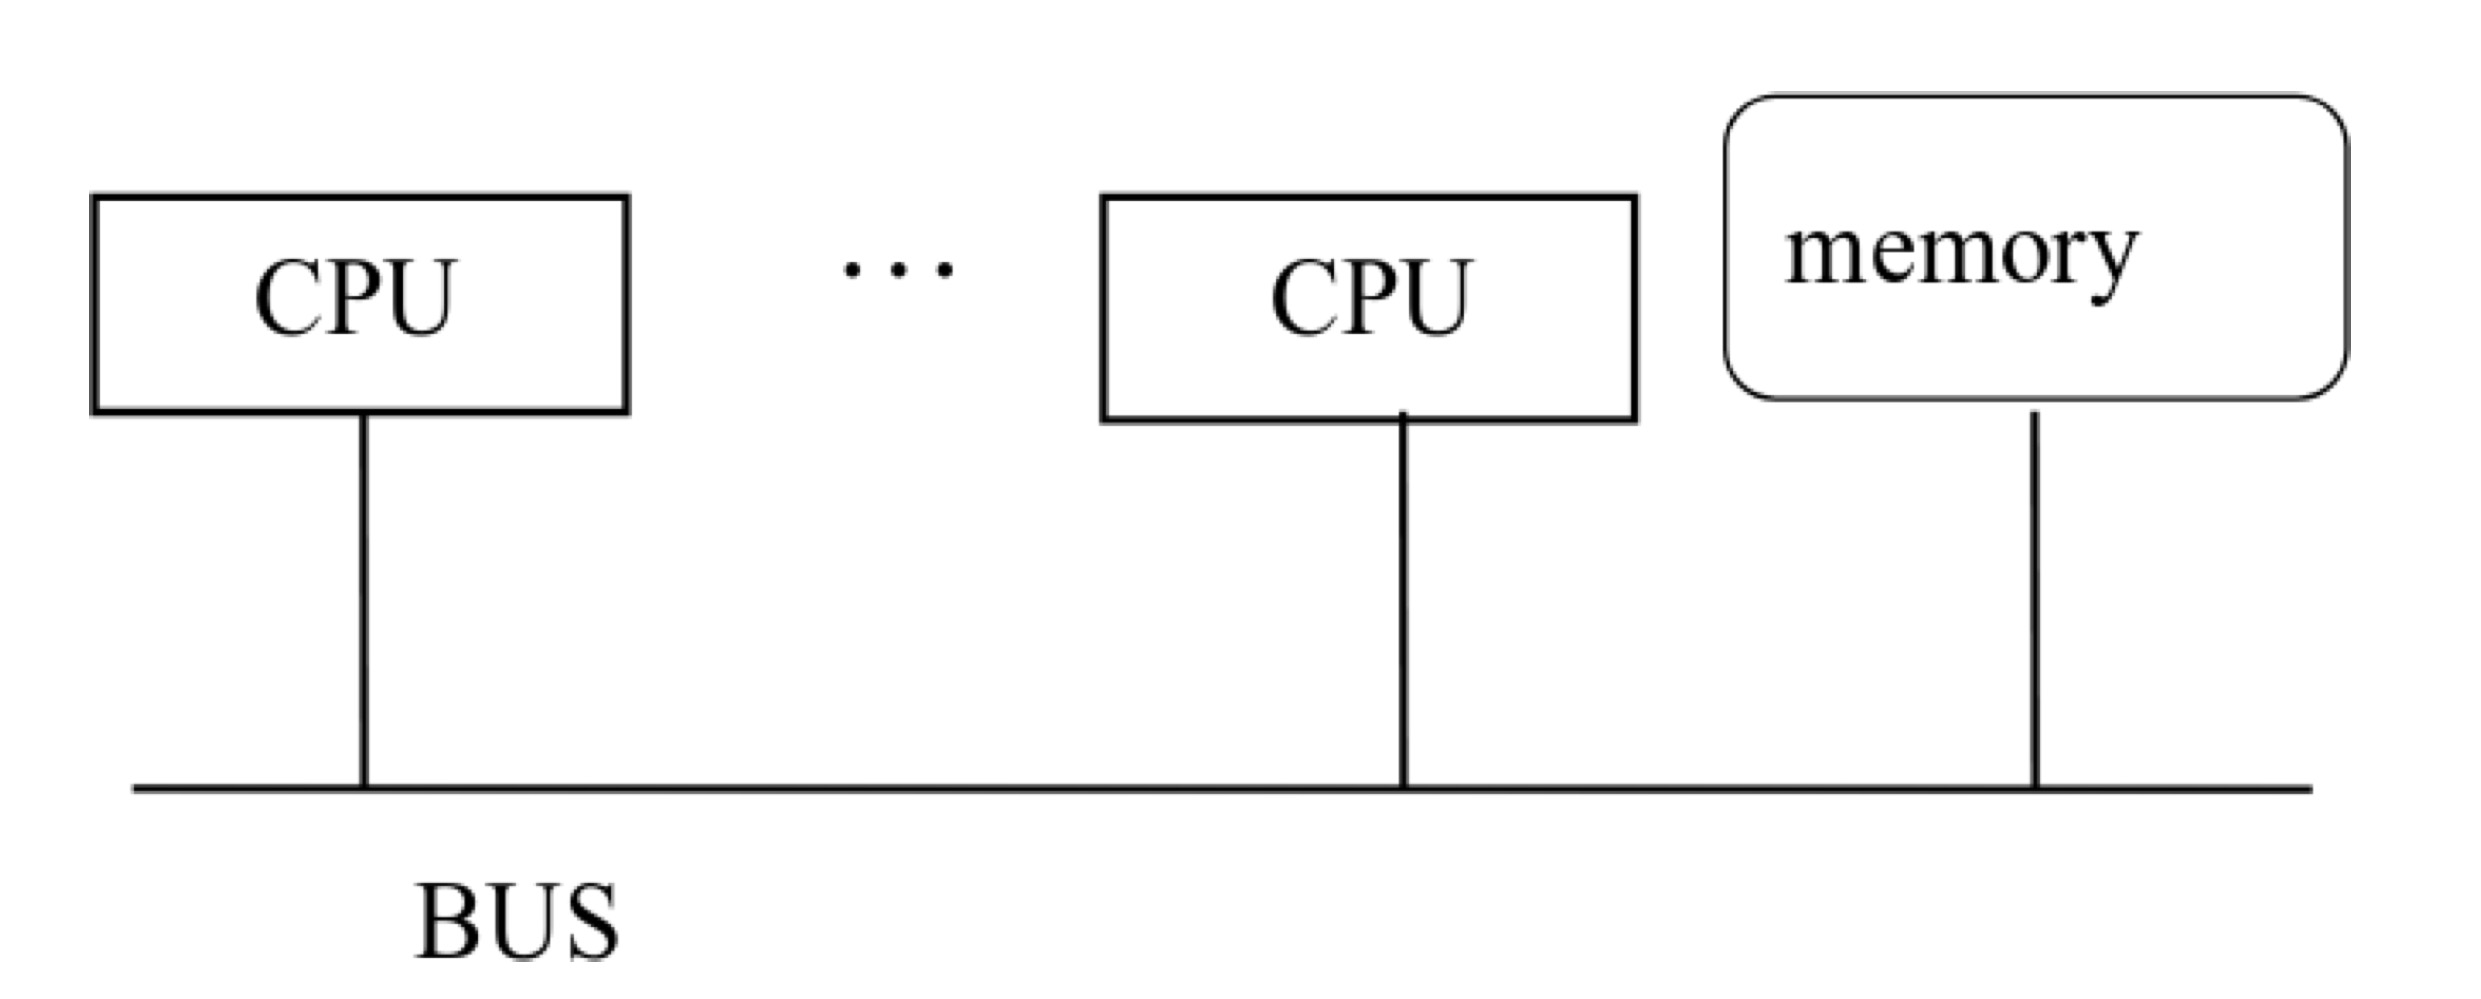
\includegraphics[width=.45\linewidth]{images/distributedSystem/busArchitecture.jpeg}
            \caption{Multiprocessor - Bus Architecture}
    \end{figure}
An improvement of this architecture is based on the \textbf{usage of a private memory}, in which each CPU has also a \textbf{private cache memory} where the most recently used words. If the required word is stored inside the cache so there is a hit and it is not necessary to access the shared memory.
The improvement is needed since there is the problem of \textbf{coherence} in which for example:
\begin{itemize}
    \item At time \(t\) CPU \(A\) writes value \(x\) at the memory address \(y\)
    \item At time \(t'\) CPU \(B\) writes value \(x\) at the memory address \(y\)
\end{itemize}
A possible solution is \textbf{write through cache}, each writing in the cache is brought to the memory. Moreover all the CPU checks for possible writing and possibly they eliminate or update the word (\textbf{snoopy cache}).
\begin{figure}
            \centering
            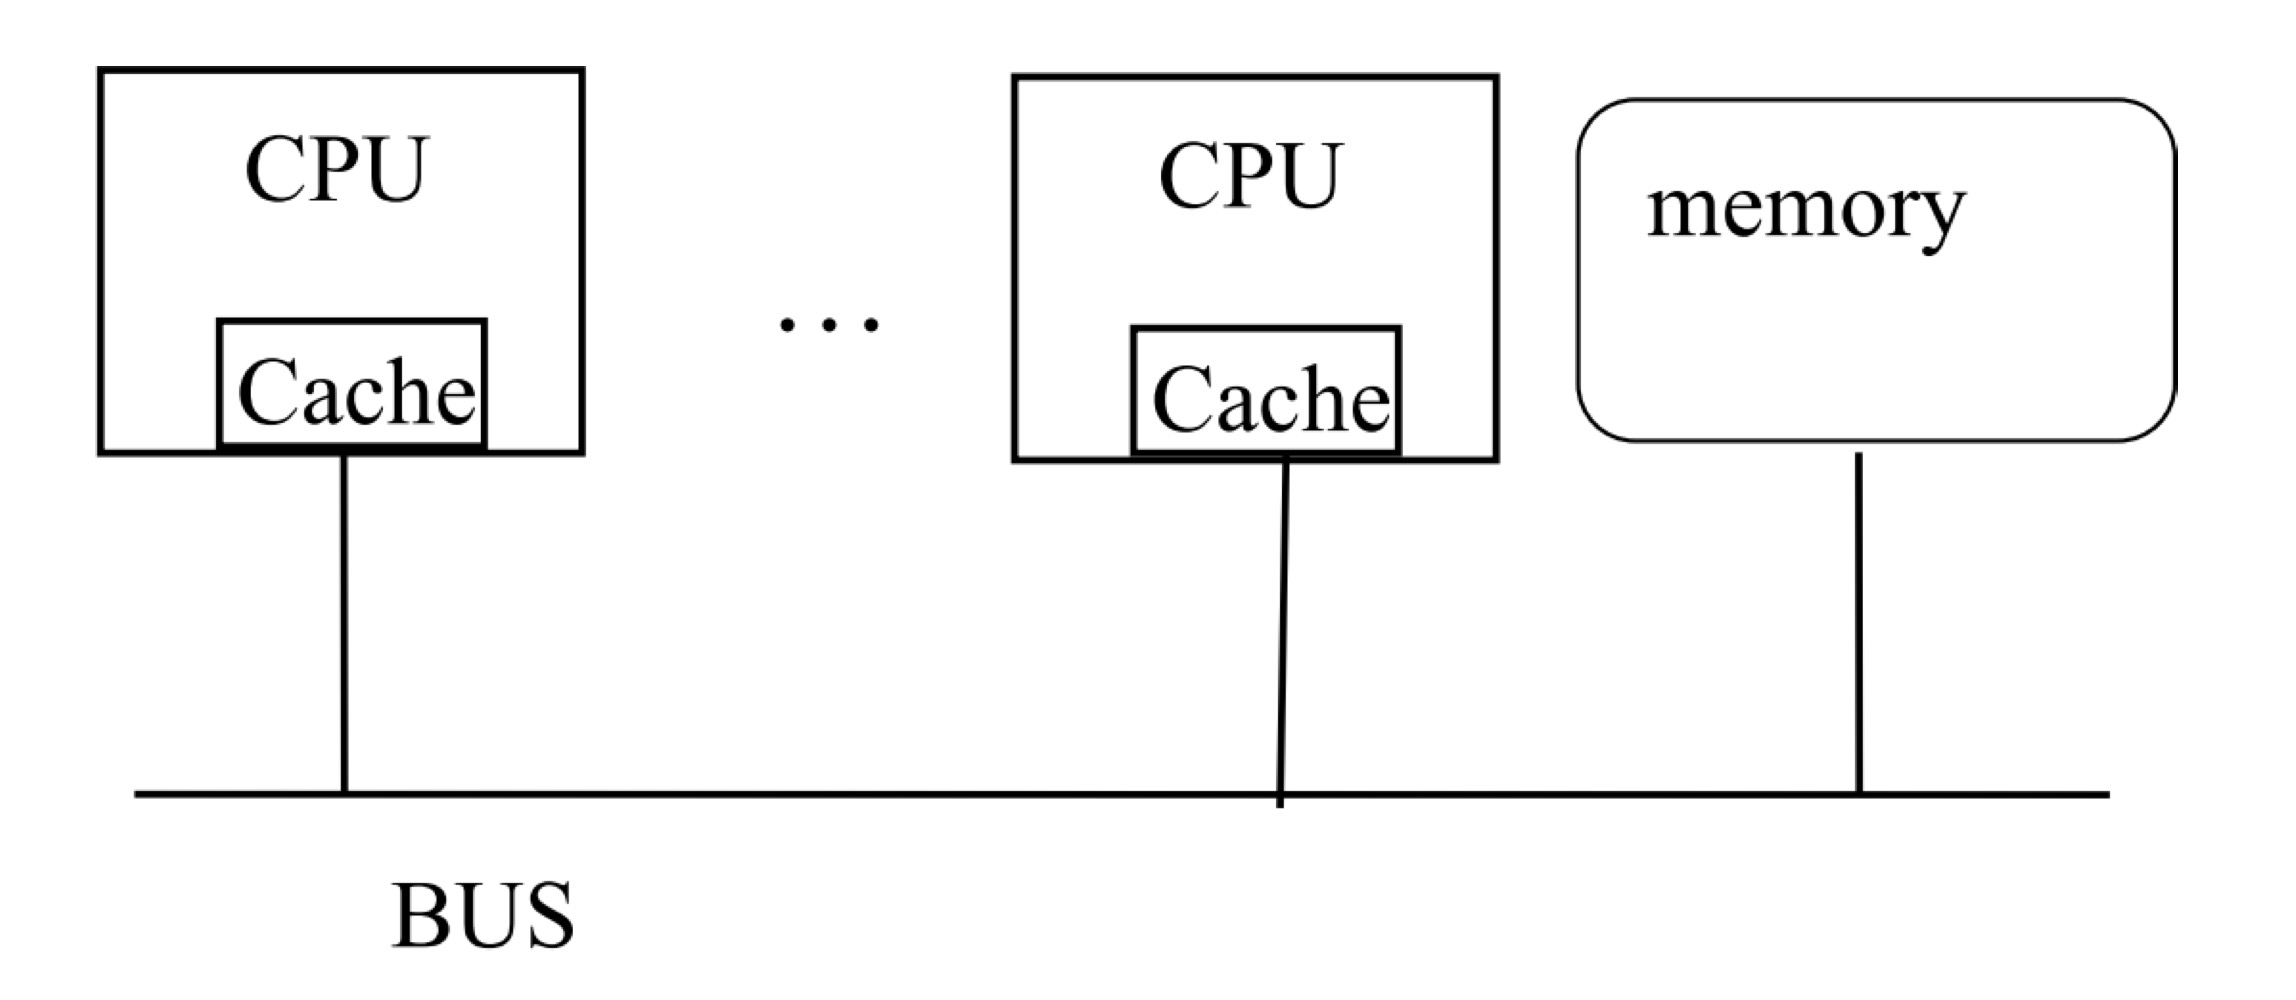
\includegraphics[width=.45\linewidth]{images/distributedSystem/busCache.jpeg}
            \caption{Multiprocessor - Bus with Cache}
    \end{figure}
\newpage
\subsection{Switch}
The \textbf{shared memory is subdivided into \(n\) modules} and a particular element, called \textbf{switch}, are used to \textit{decide the right path.} With this implementation different CPUs can access different memory modules at the same time. N memory modules and N CPUs require \(N^2\) switches. If all CPUs want to access the first memory we have the \textbf{array-like case}, otherwise we could introduce some sort of parallelisms
\begin{figure}[!h]
            \centering
            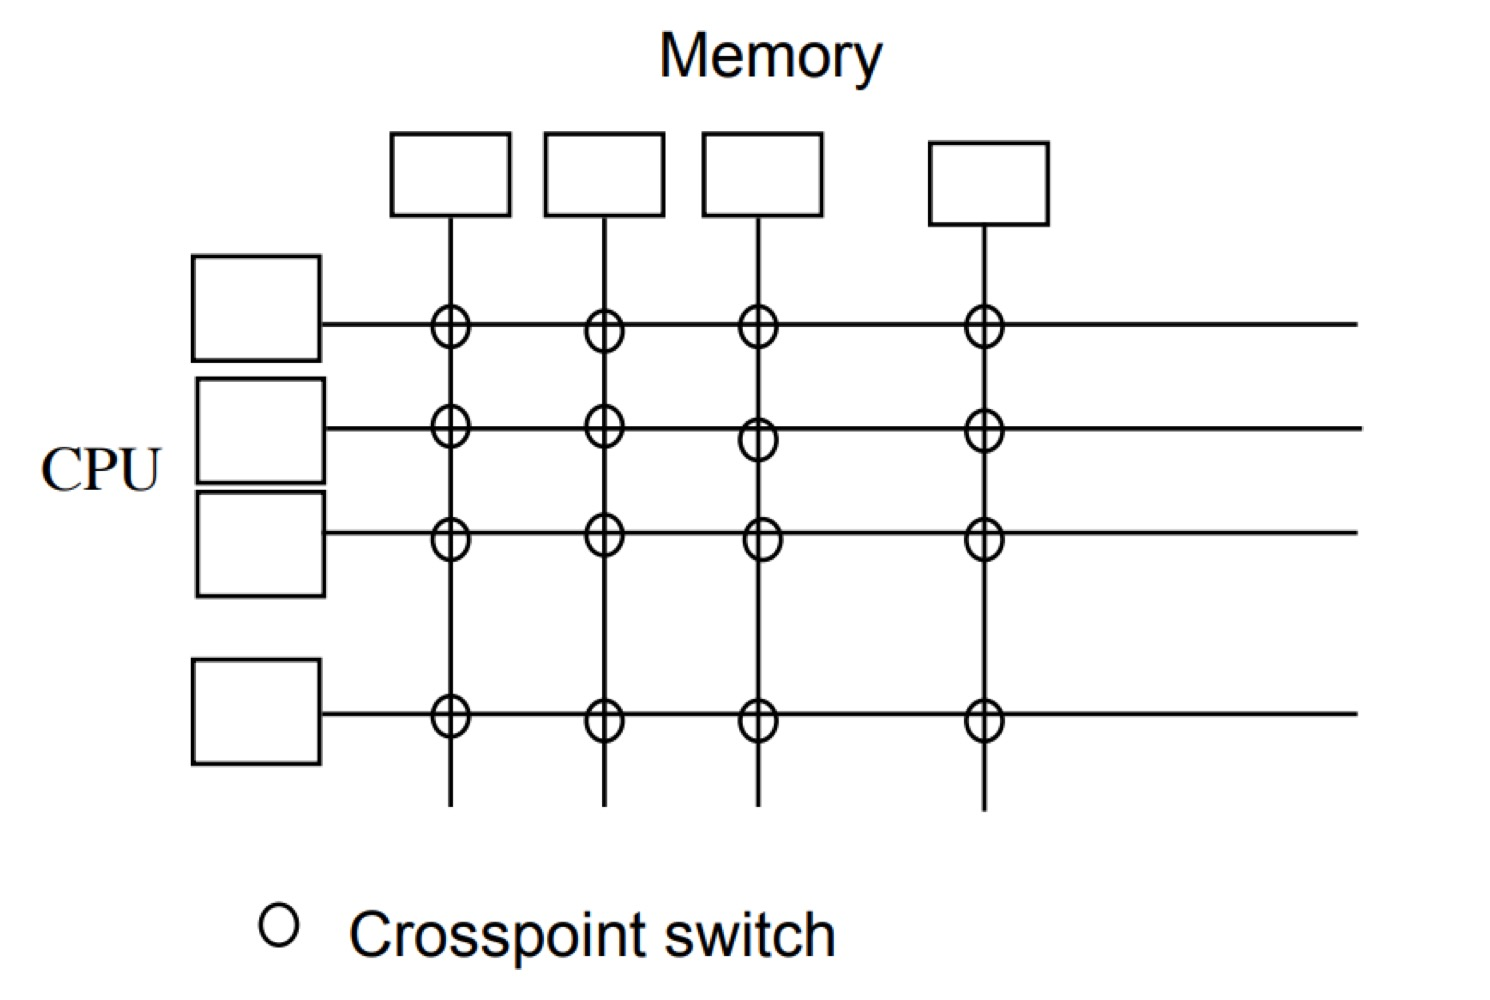
\includegraphics[width=.45\linewidth]{images/distributedSystem/switch.jpeg}
            \caption{Multiprocessor - Switch}
    \end{figure}

\subsection{Omega Network}
Respect to switch architecture, switches are organized as a \textbf{binary tree} with direct access from each CPU to each module, so there is a \textbf{decreasing number of switches} \((\frac{n}{2} \log n)\). But the \textbf{drawback} is the \textit{communication delay} of each switch.
\begin{figure}[!h]
            \centering
            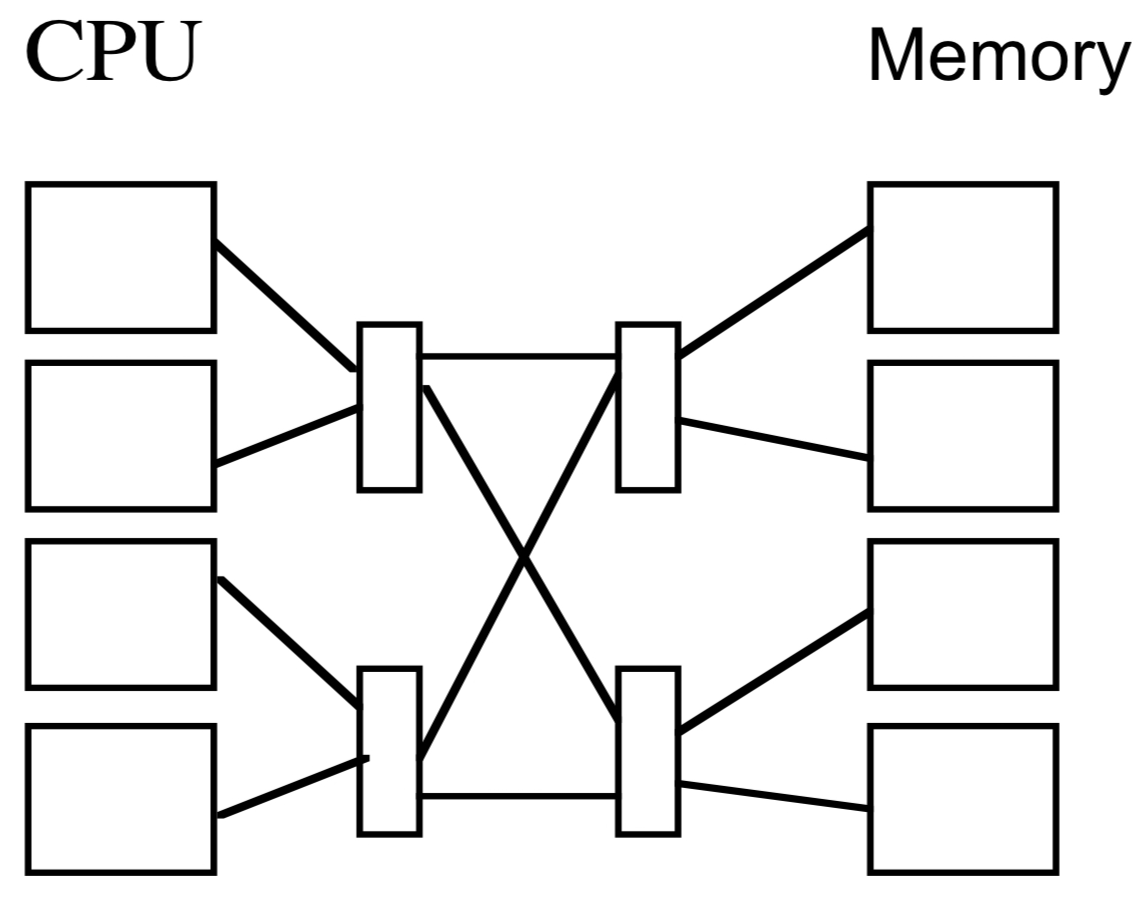
\includegraphics[width=.35\linewidth]{images/distributedSystem/numa.jpeg}
            \caption{Multiprocessor - Omega}
    \end{figure}

\subsection{NUMA}
NUMA (Not Uniform Memory Access), \textbf{each CPU has a local memory}, this brings an \textbf{increase of performance} since CPUs save most of the data of shared memory inside local memory. It is necessary to develop an allocation algorithm for programs and data. 


\section{Multicomputer}
\begin{itemize}
    \item Each computer system is composed of a \textbf{private local memory}
    \item They can be local at different positions, loosely coupled, so:
    \begin{itemize}
        \item Longer transmission delay
        \item Lower transmission speed
    \end{itemize}
    \item The computer systems are \textbf{autonomous}
    \item They are \textbf{connected by a network} and they interact using it
\end{itemize}
Also here there can be different architectures:
\subsection{Bus}
Computer systems are connected by a \textbf{bus line} but there is \textbf{no shared memory}. They can \textit{access remote resources}. It is necessary to implement a system to reduce traffic and some communication network protocols.
\begin{figure}[!h]
            \centering
            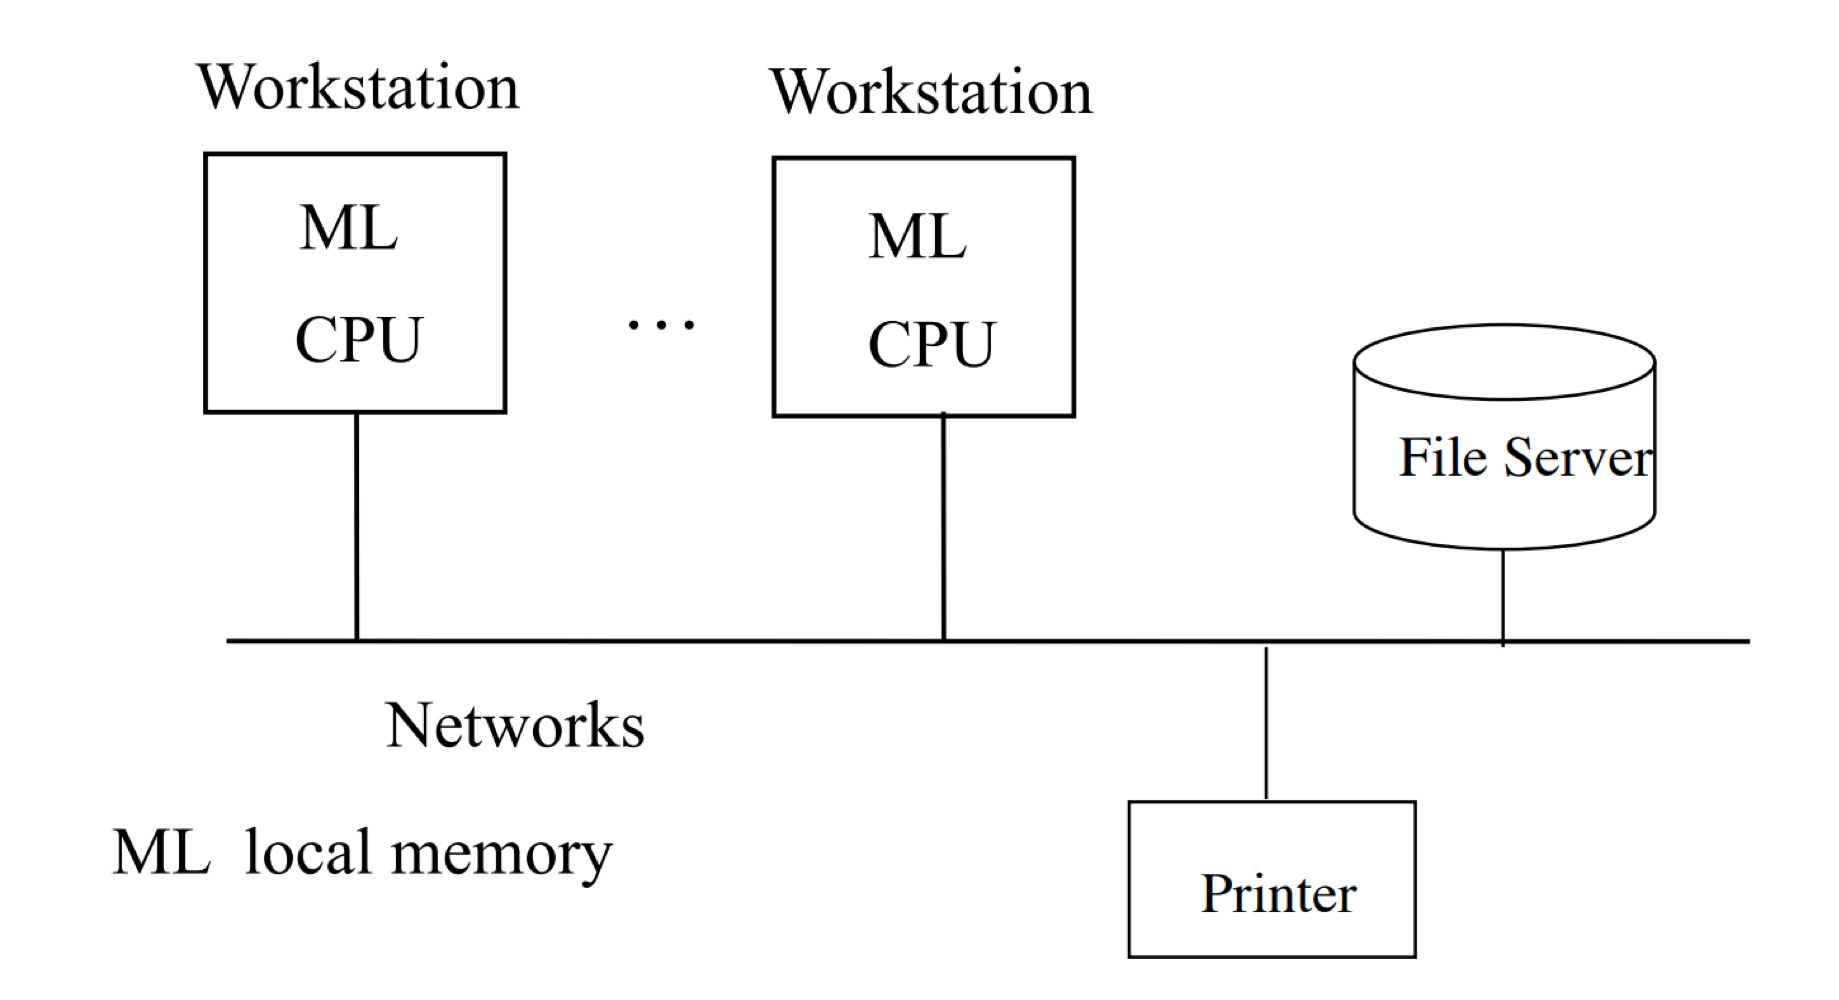
\includegraphics[width=.45\linewidth]{images/distributedSystem/multicomputerBus.jpeg}
            \caption{Multicomputer - Bus}
    \end{figure}
    
\subsection{Switch}
Computer systems can be organized as a \textbf{grid of switches or hypercubes}, that reduces the number of steps and switches necessary to connect all the nodes.
\begin{figure}[!h]
            \centering
            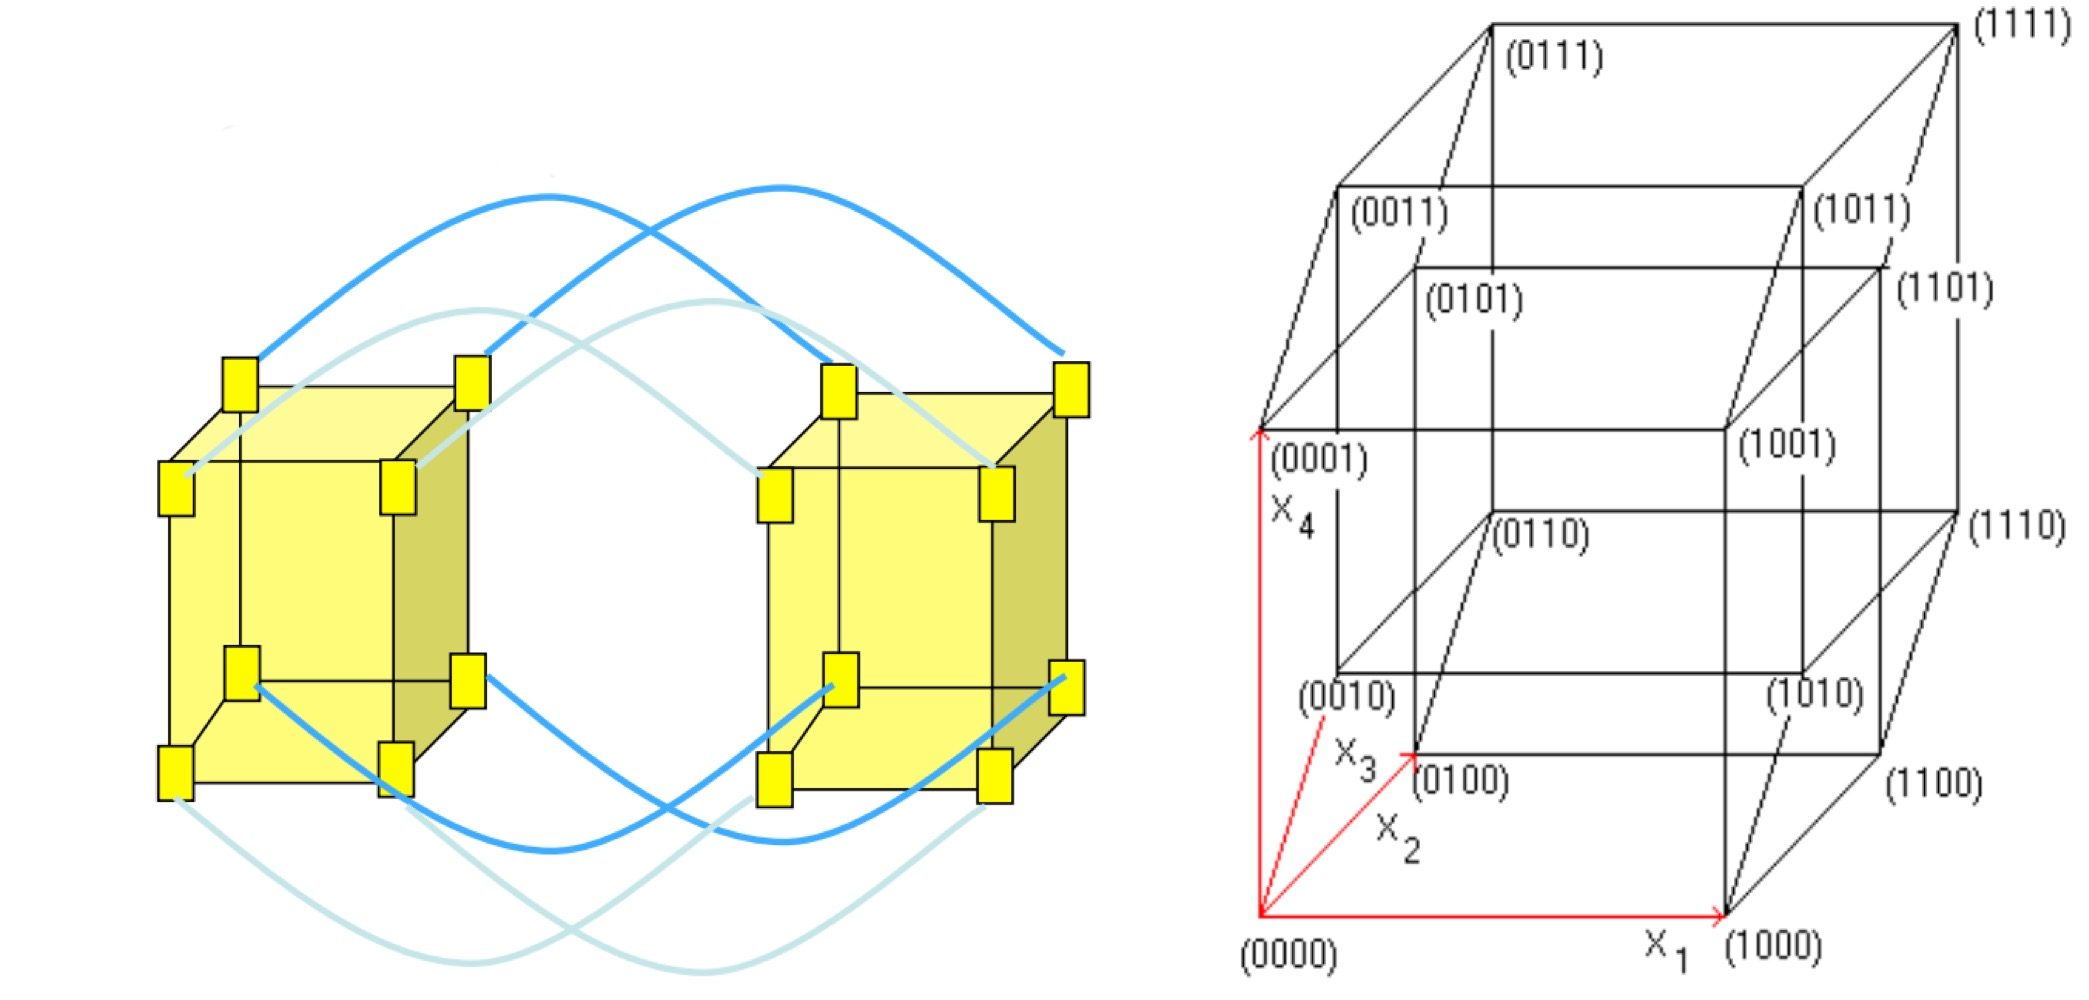
\includegraphics[width=.7\linewidth]{images/distributedSystem/multipcSwitch.jpeg}
            \caption{Multicomputer - Switch}
    \end{figure}
    
    
\section{Type of Distributed System}
\begin{itemize}
    \item \textbf{Systems with massive parallelism}, like supercomputers with thousands of CPUs, which have \textit{low latency, high bandwidth and good reliability}
    \item Systems with \textbf{clusters of workstations (COW)}, computer systems connected with available components. There is  no special design to optimise performance and reliability. Like homogeneous systems.
    \item \textbf{Cloud computing systems:} in which there are computers as utility, resource visualisation, on demand feature, pay-per-use model, high scalability and transparency
    \item \textbf{Distributed transaction processing systems:} like database applications
    \item \textbf{Pervasive, ubiquitous, mobile systems}
    \item \textbf{Sensor networks:} energy critical systems
\end{itemize}
\begin{figure}[!h]
            \centering
            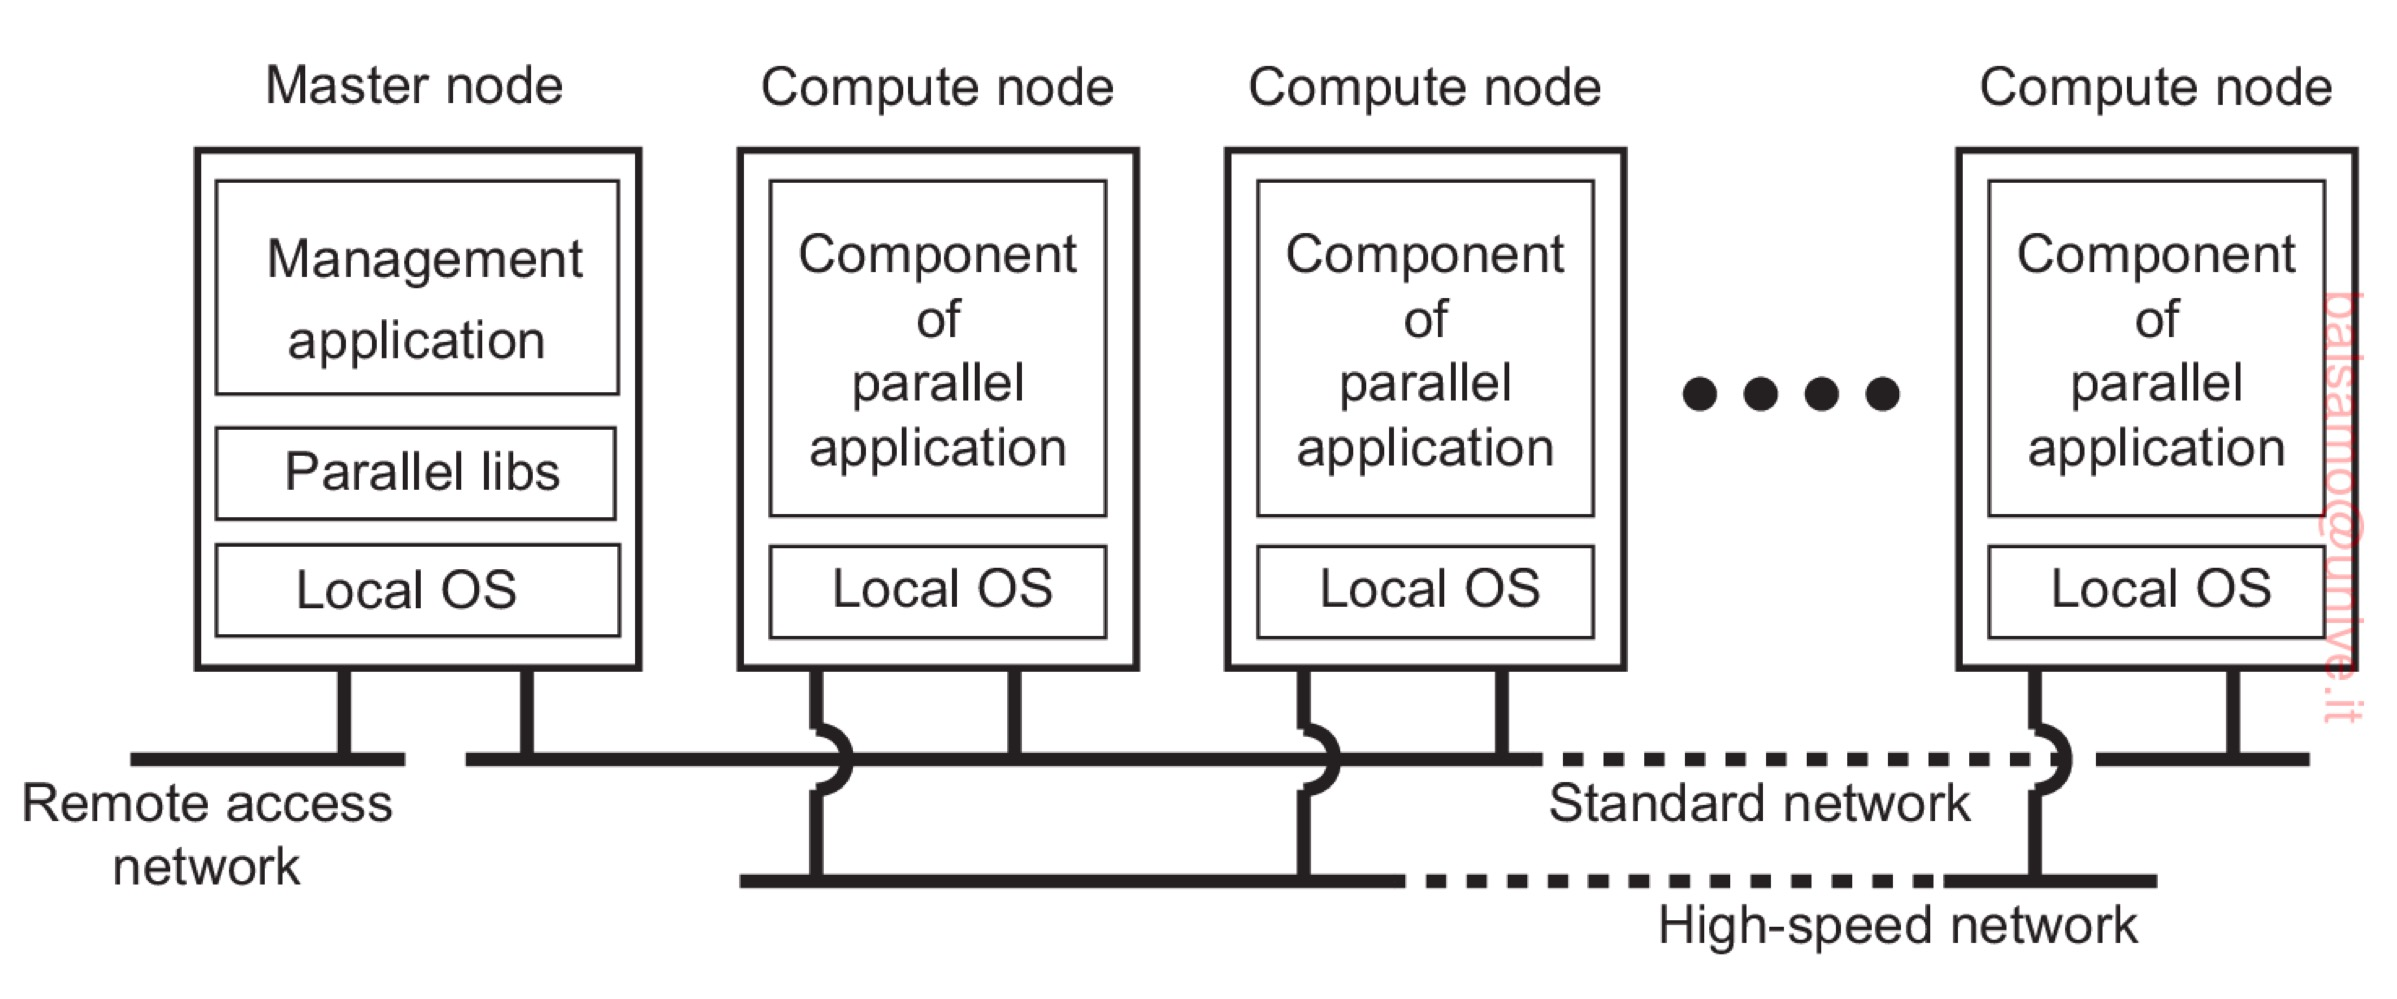
\includegraphics[width=.7\linewidth]{images/distributedSystem/typeOfDS.jpeg}
            \caption{Example of a cluster of computer systems. A single program can run in parallel on a set of c.s.
Master: process allocation, user interface and Compute nodes: use the middleware 
}
    \end{figure}
    
\begin{figure}[!ht]
            \centering
            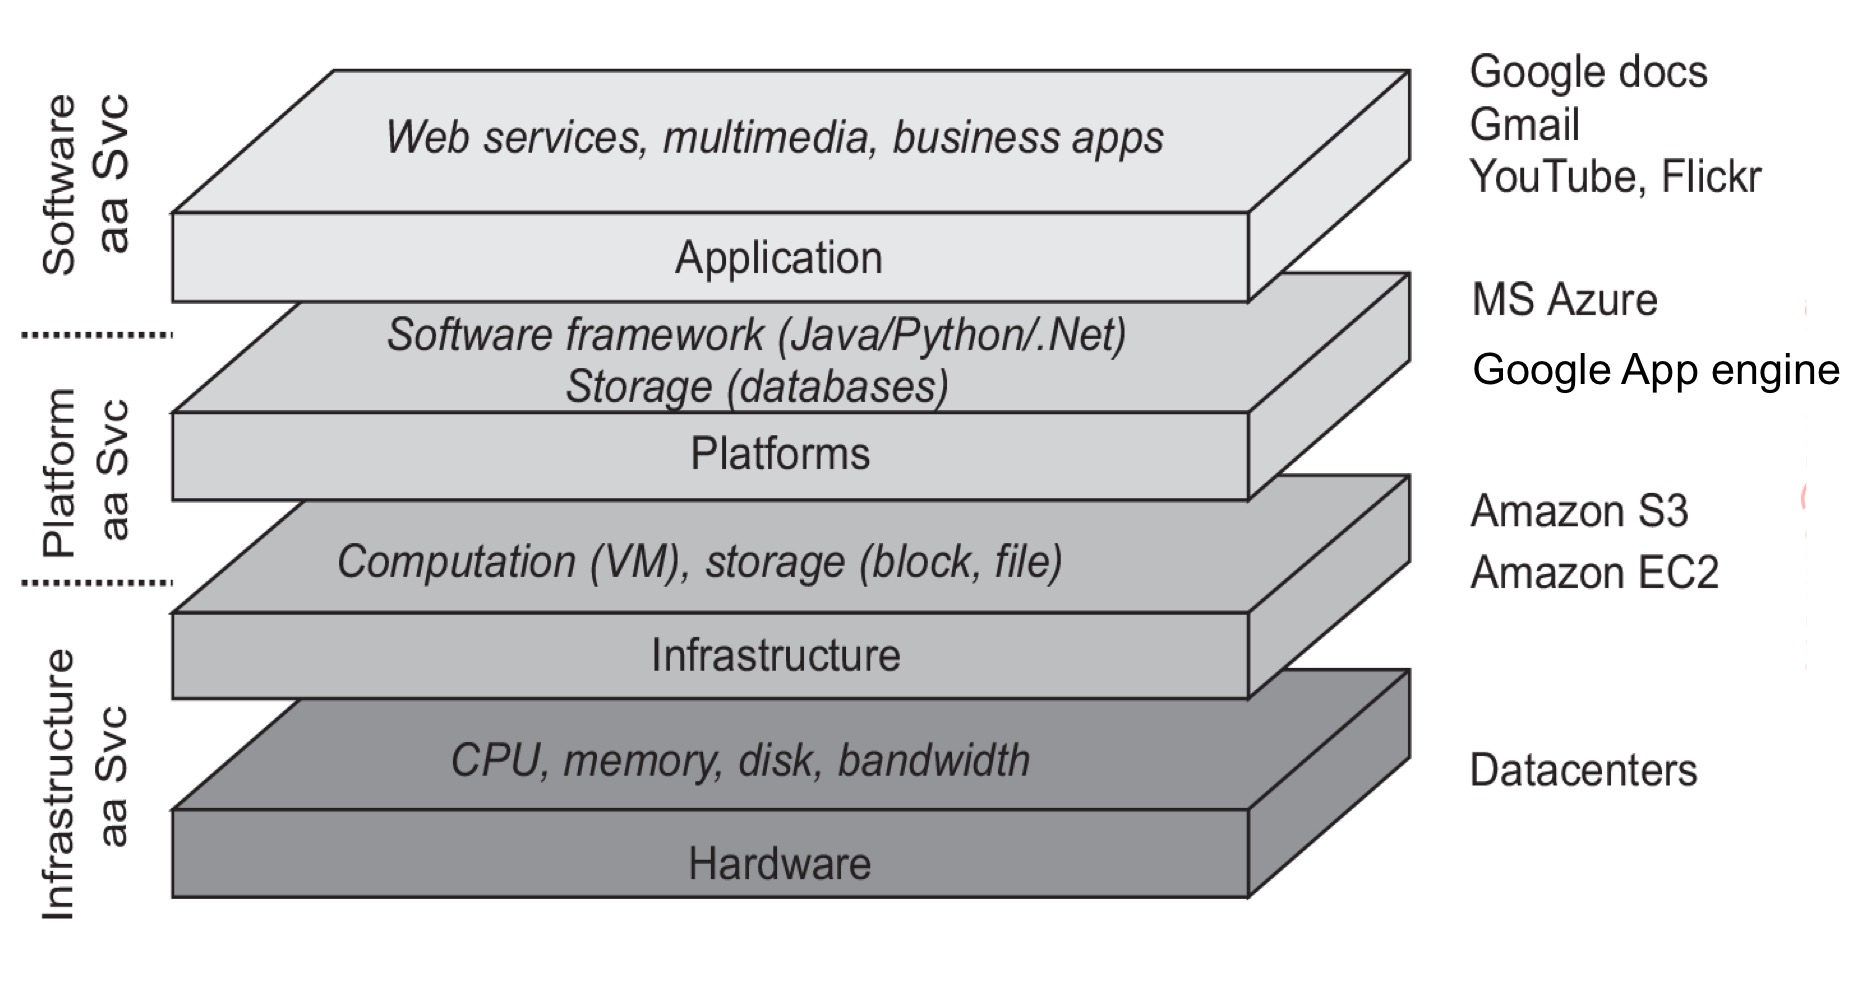
\includegraphics[width=.7\linewidth]{images/distributedSystem/CCdefinition.jpeg}
            \caption{Organization of cloud computing - levels of services - Example
}
    \end{figure}
    
\section{Software Organization}
A distributed system can be classified also based on the software architecture adopted:
\begin{itemize}
    \item \textbf{Loosely-coupled:} in which machines are \textbf{completely independent and they share resources.} Each computer system can be identified and it is able to operate independently of others in such a way that a network fault does not block the operation of a single computer system
    \item \textbf{Tightly-coupled,} machines are \textbf{independent} but there is a \textbf{controller} that coordinates them. We can say that there exists a hierarchy structure.
\end{itemize}
We can distinguish several Operating Systems depending on the type of the system we are dealing with:
\begin{itemize}
    \item \textbf{Uniprocessor system:} for a single central system the OS provides the virtualization of the machine and manages the resources and processes. The model for the OS can be classified in two categories:
    \begin{itemize}
        \item \textbf{Microkernel} model which is made by layered components, in such a way that upper components provide functionalities to the lower parts.
        \item \textbf{Monolithic} model in which all the components are stored.
    \end{itemize}
    \item \textbf{Network management in a distributed system (NOS, LCS - LCH):}  has \textbf{loosely coupled software} on a \textbf{loosely coupled hardware}. It’s a network of machines each with its own memory, CPU, OS and devices. The remote execution requires that the job can see the resource location
    \begin{figure}[!h]
            \centering
            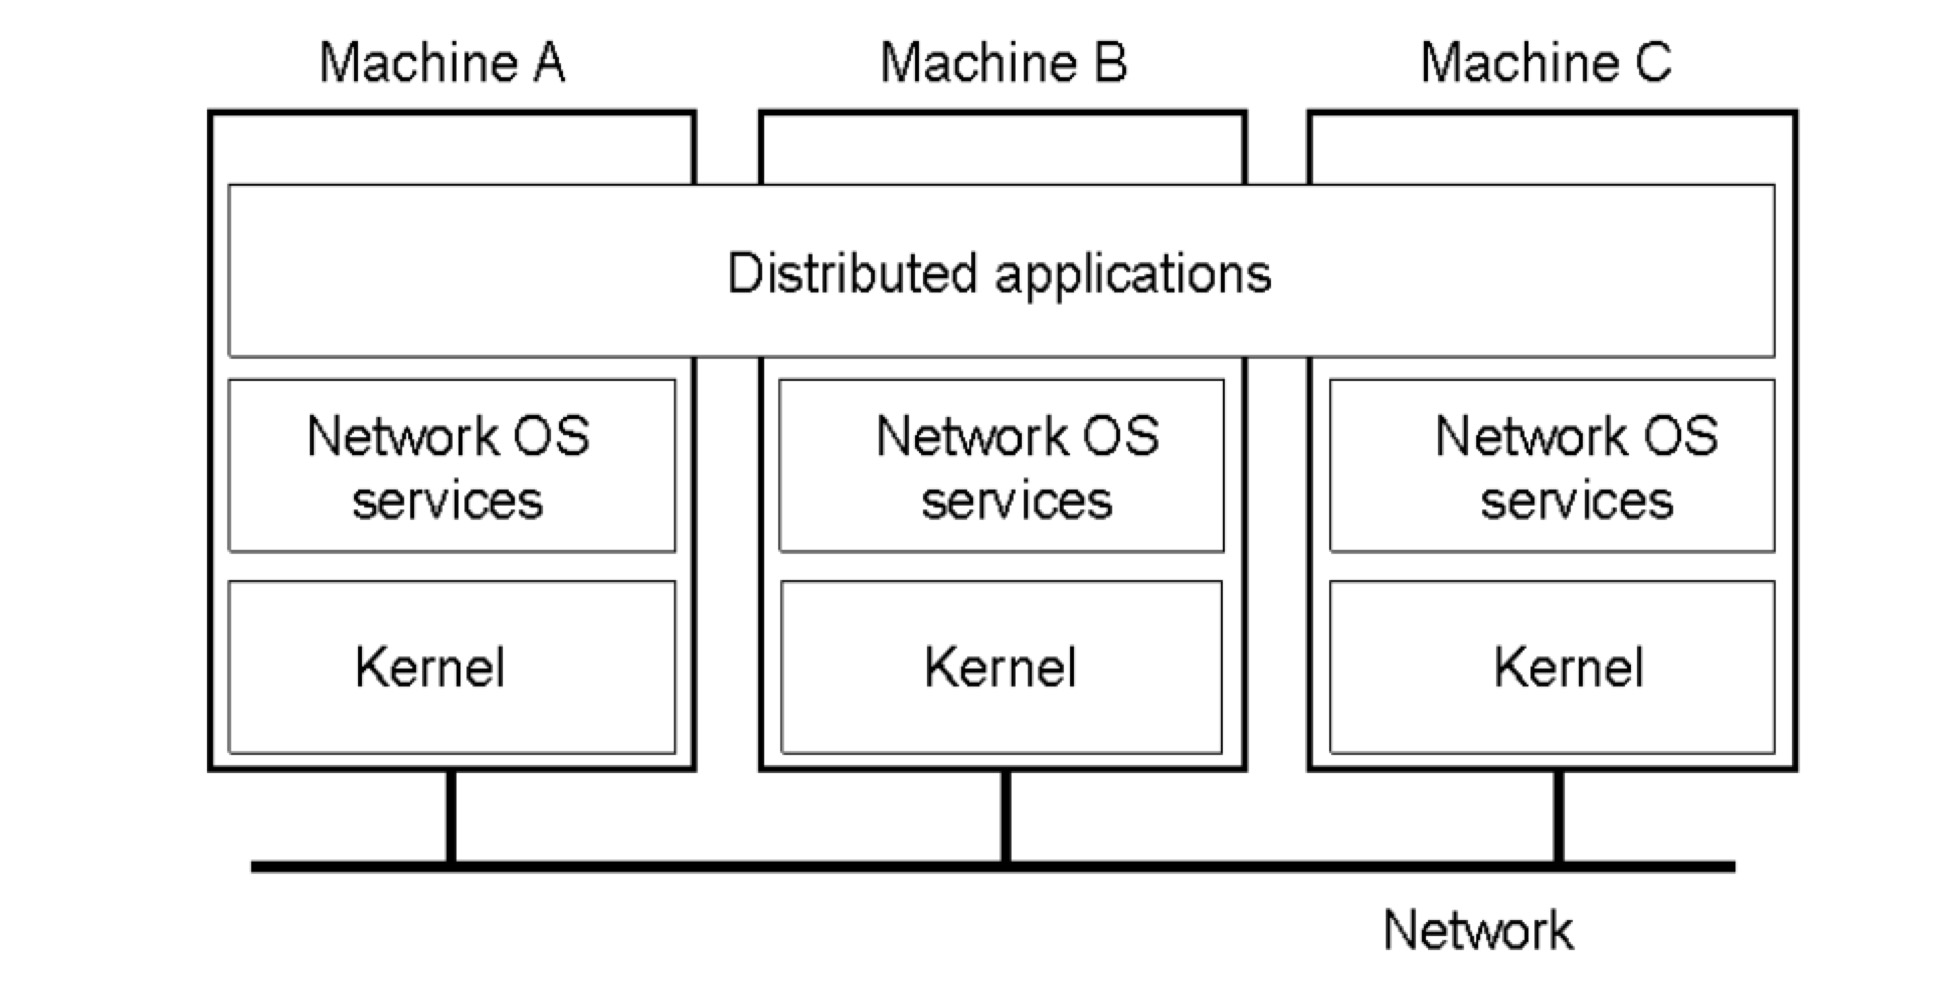
\includegraphics[width=.6\linewidth]{images/distributedSystem/NOSArchitecture.jpeg}
            \caption{NOS Architecture}
    \end{figure}
    \item \textbf{Distributed system (DOS, TCS - LCH):} has a \textbf{tightly coupled software} on a \textbf{loosely coupled hardware}. 
    \begin{itemize}
        \item Everything is managed by a \textbf{global manager, without sharing memory.}
        \item It is an operating system that produces a single system image for all the resources.
        \item A DOS is an operating system that runs on \textbf{several machines} whose purpose is to provide a useful set of services.
        \item DOS also has the role in making the collective resources of the machines more usable
        \item Usually, the machines controlled by a distributed operating system are connected by a relatively high quality network, such as a high speed local area network.
        \item A DOS should provide:
        \begin{itemize}
            \item Common IPC, provides mechanisms to allow the processes to \textbf{manage shared data}
            \item \textbf{Global protection}, provides protection mechanisms to maintain secure systems and data
            \item \textbf{Process management}, which provides mechanisms to manage processes
            \item \textbf{File system}, allows a unique view and access way to the file system
            \item \textbf{System interface}, gives a unique and homogeneous interface to give the maximum transparency
        \end{itemize}
    \end{itemize}
    \begin{figure}[!h]
            \centering
            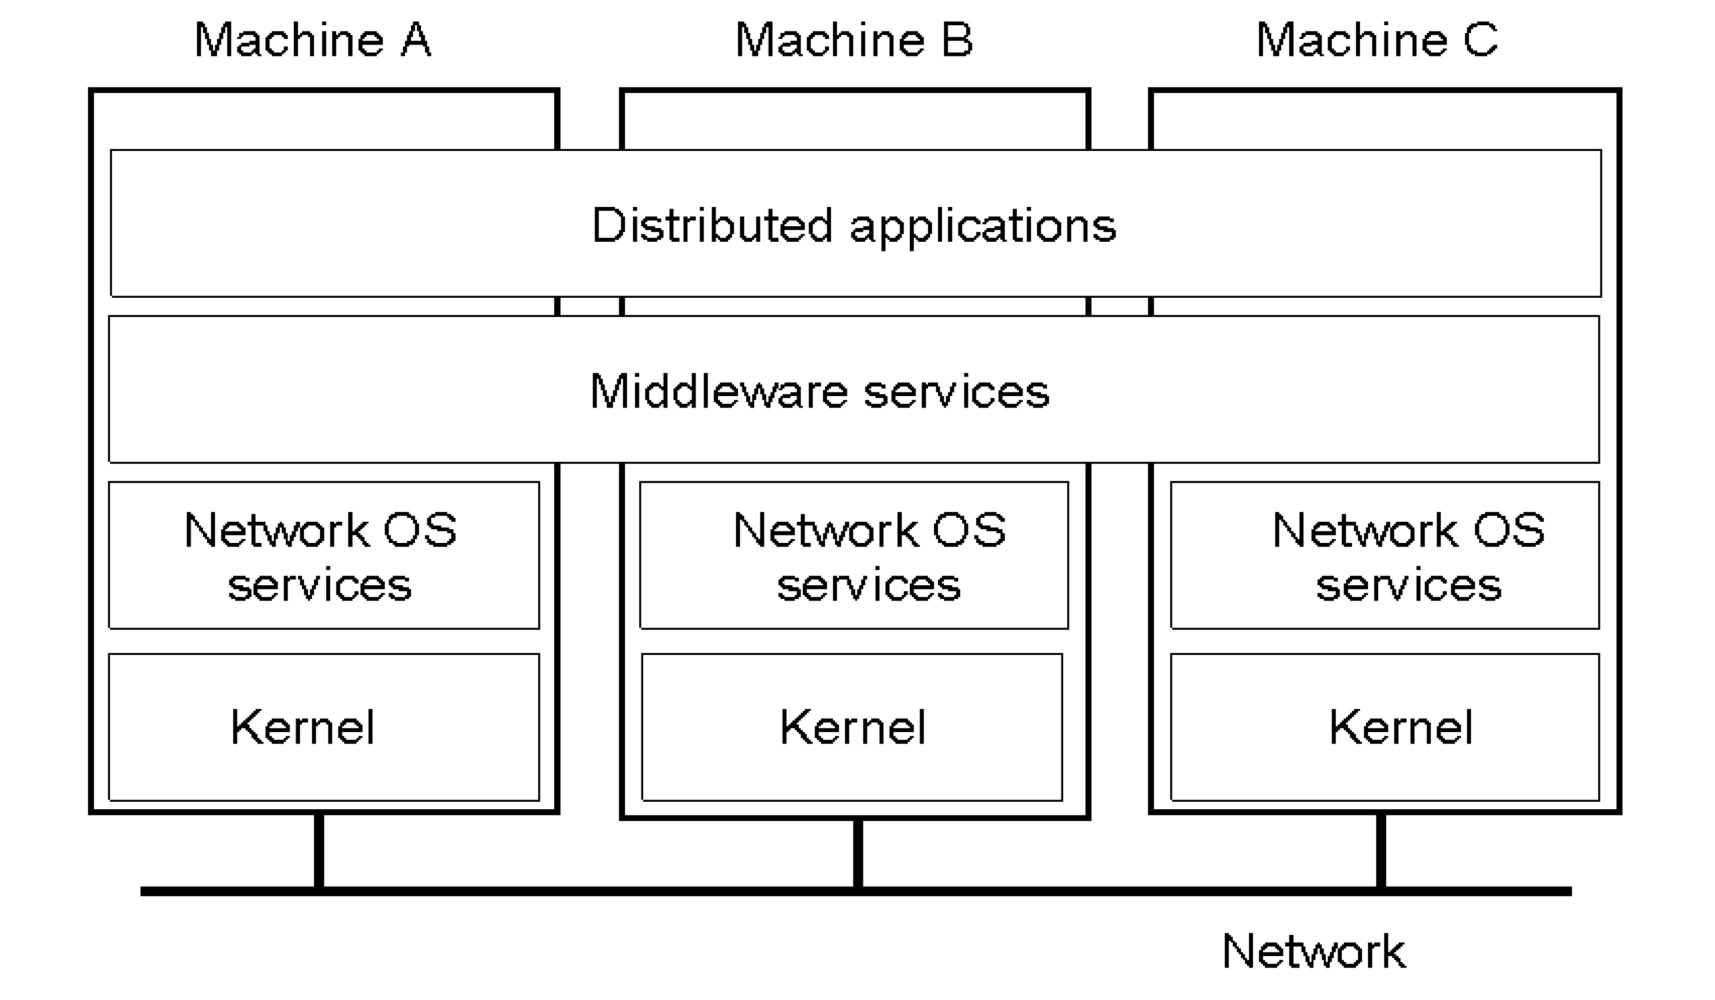
\includegraphics[width=.6\linewidth]{images/distributedSystem/DOSArchitecture.jpeg}
            \caption{DOS Architecture}
    \end{figure}
    \begin{figure}[!htb]
       \begin{minipage}{0.48\textwidth}
         \centering
         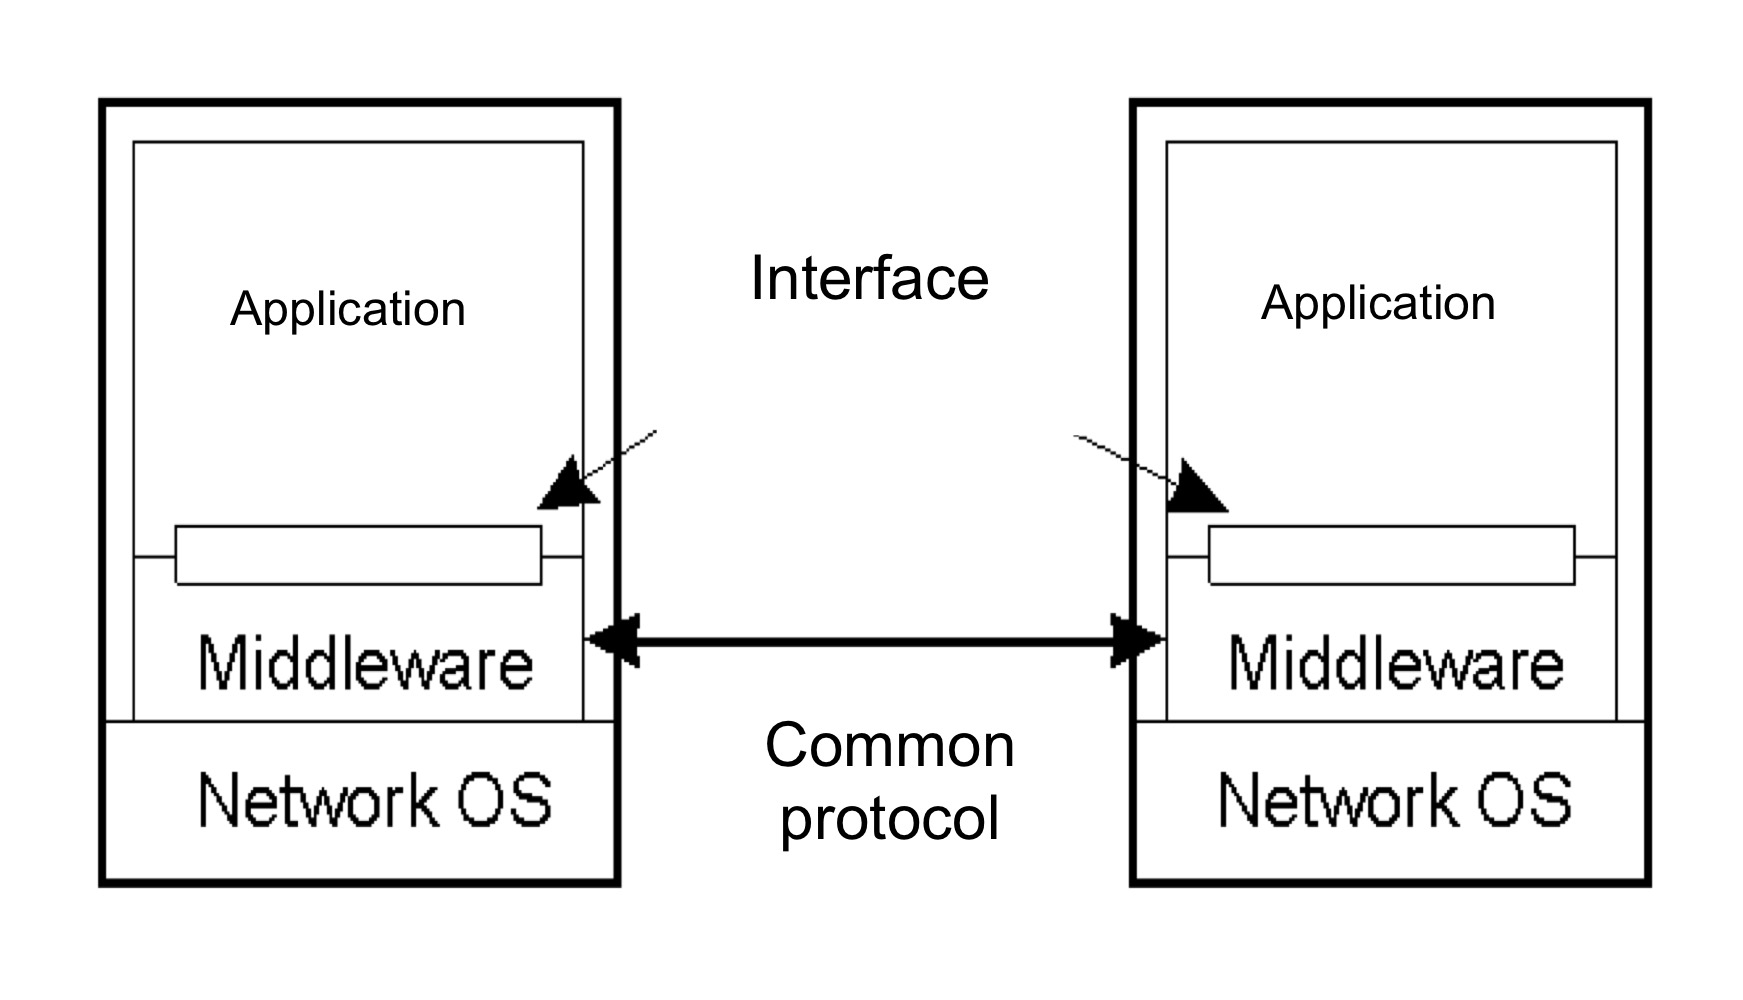
\includegraphics[width=.7\linewidth]{images/distributedSystem/middleware1.jpeg}
         \caption{In an open distributed system based on \textbf{middleware}  the used protocol by each middleware level should be the same. Like the offered \textbf{interface}s to the application}
       \end{minipage}\hfill
       \begin{minipage}{0.48\textwidth} 
         \centering
         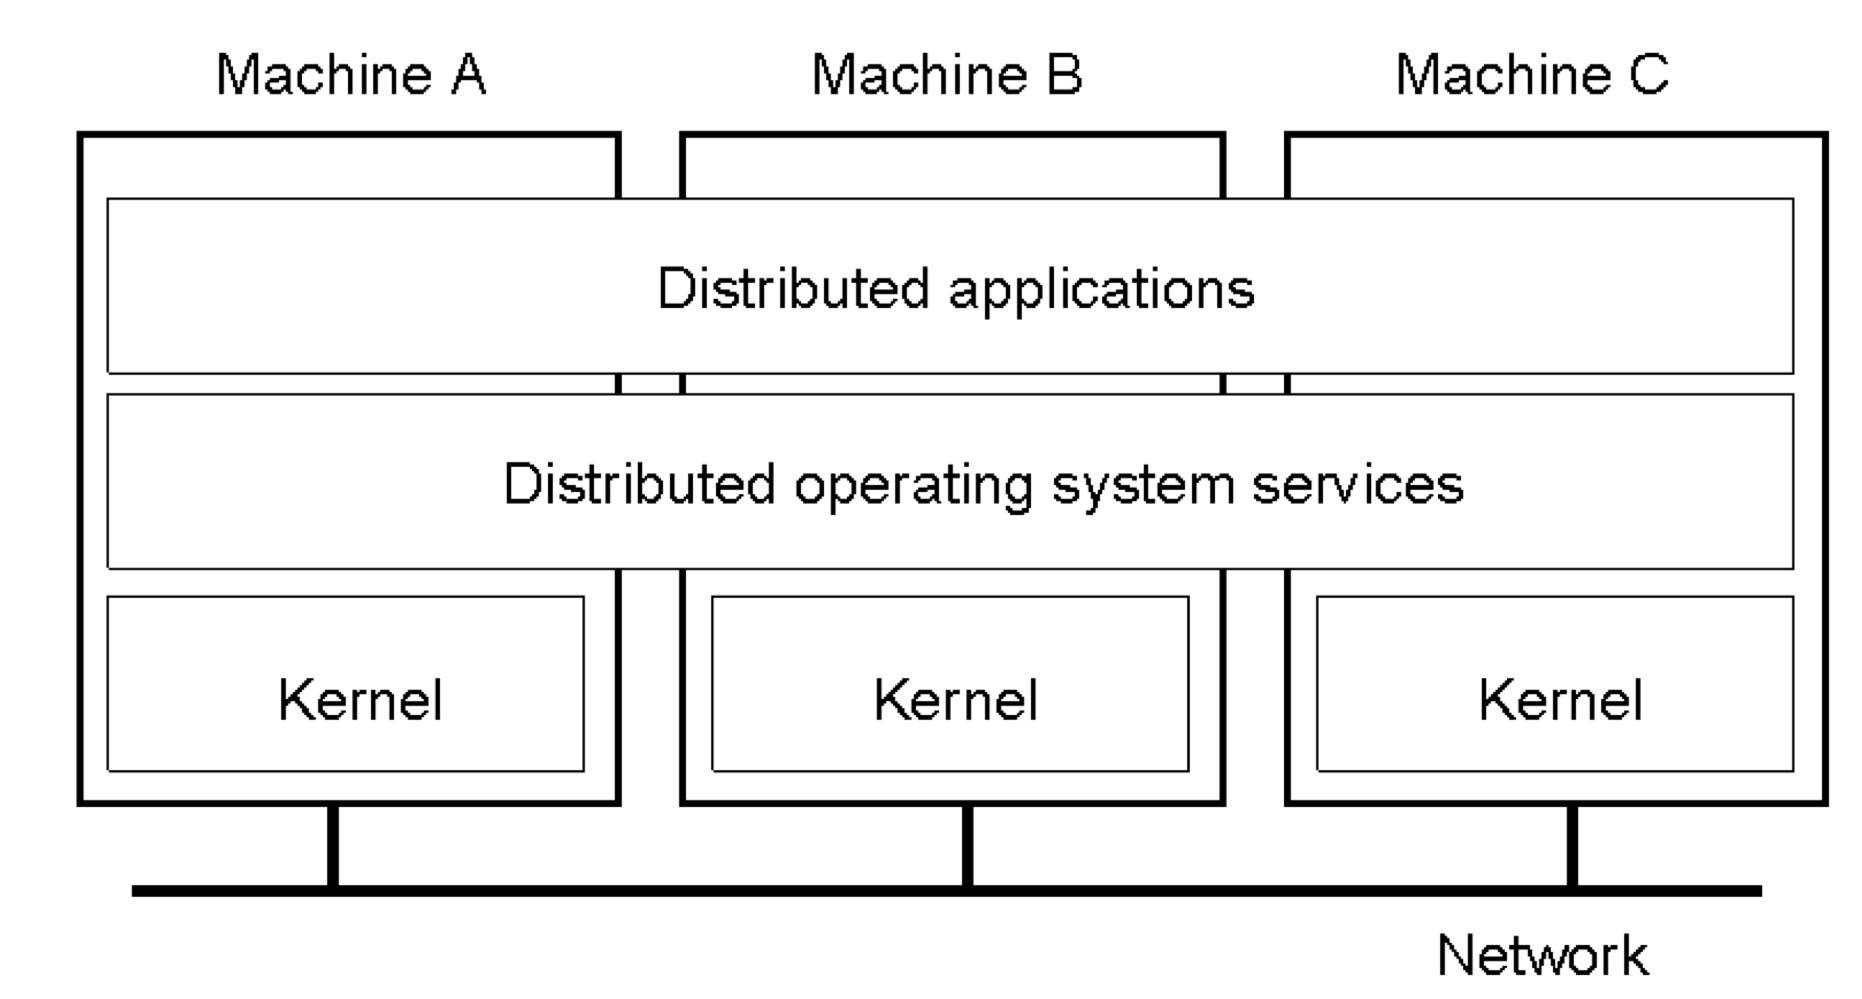
\includegraphics[width=.7\linewidth]{images/distributedSystem/middleware2.jpeg}
         \caption{General structure of \textbf{multicomputer} operating system}
       \end{minipage}
    \end{figure}
    \item \textbf{Multiprocessor system (MOS, TCS - TCH):}  has a \textbf{tightly coupled software} on a \textbf{tightly coupled hardware.}
    \begin{itemize}
        \item It has a \textbf{global shared memory} 
        \item There is a \textbf{unique global execution queue} and several \textbf{CPUs} that execute ready processes
        \item In order to have an advantage from the presence of the cache it’s important that the \textbf{scheduler considers also in which CPU have already run processes ready for the execution.}
    \end{itemize}
    \begin{figure}[!h]
            \centering
         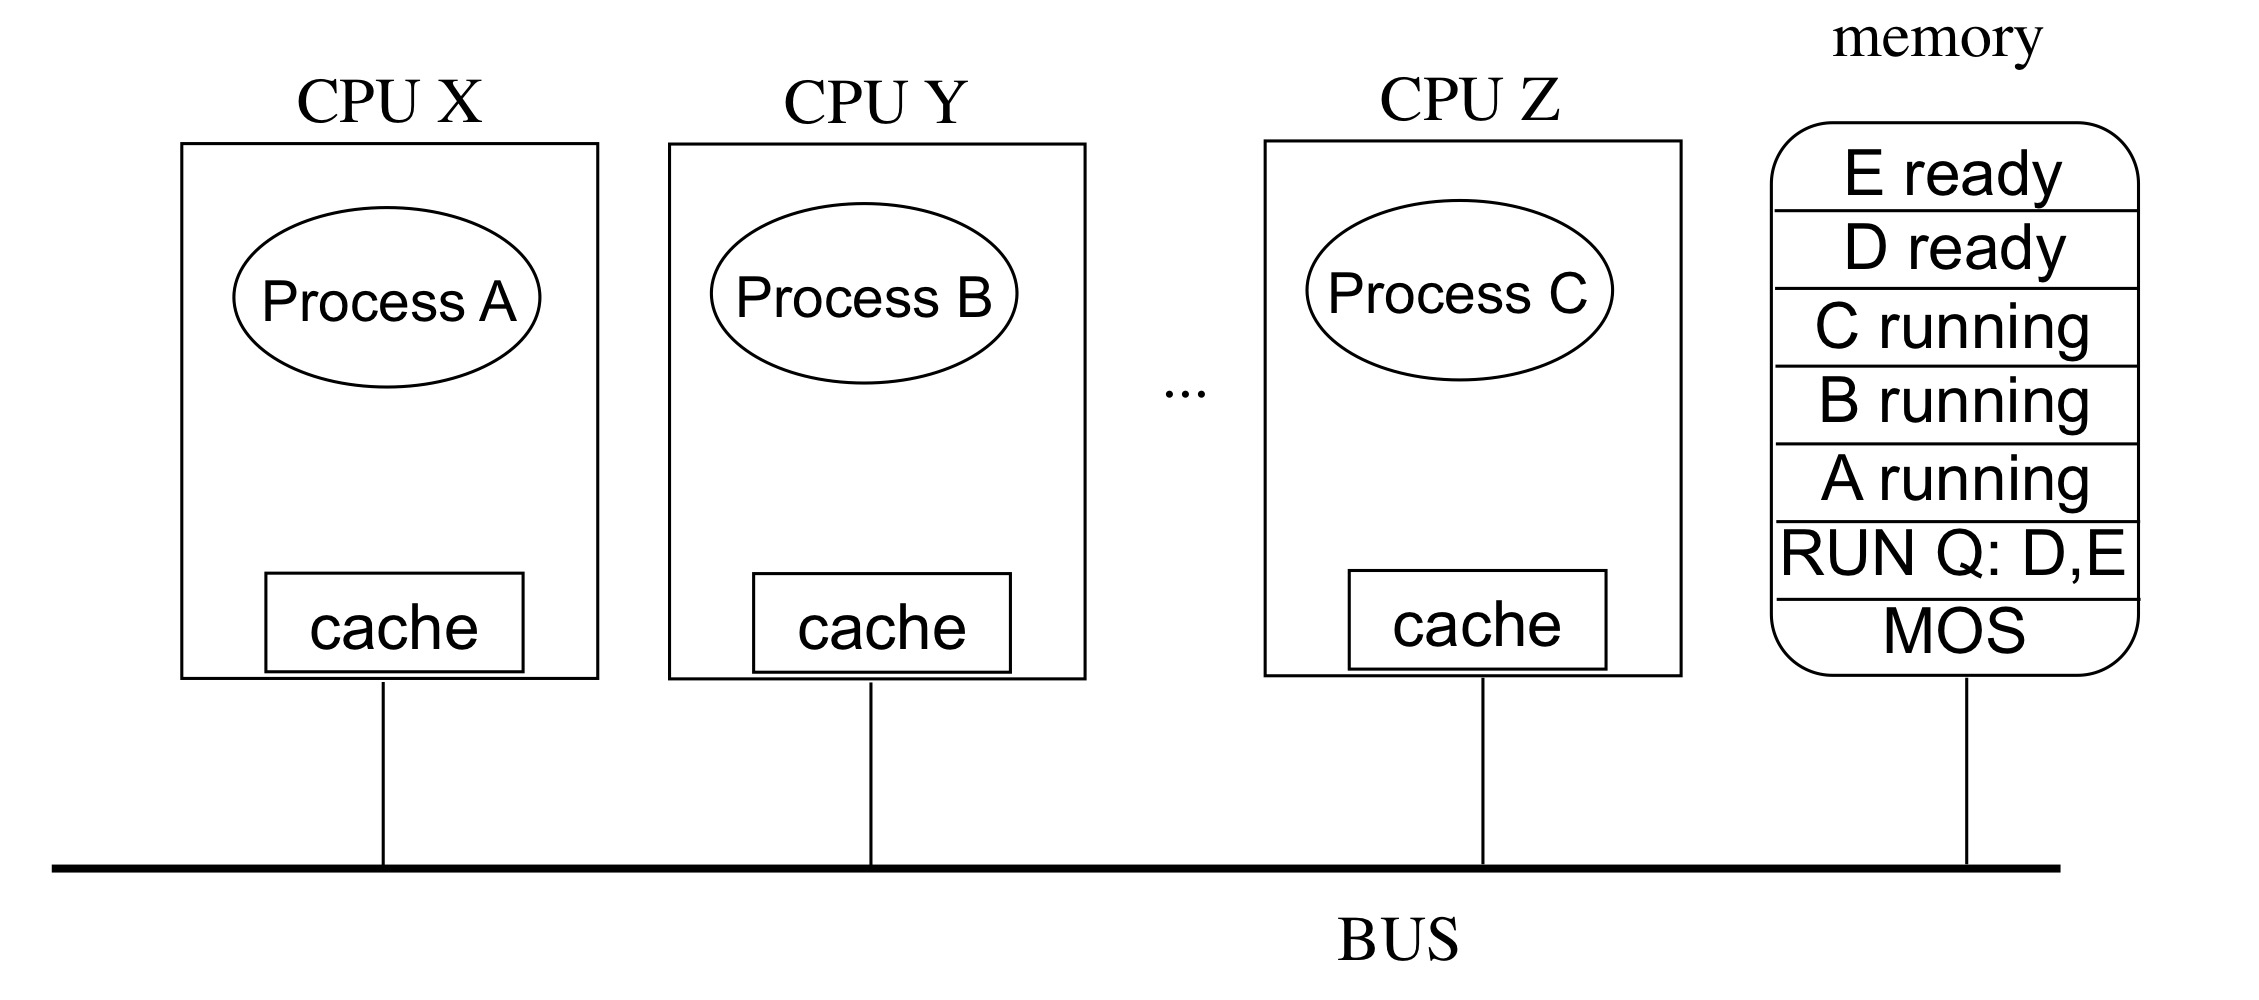
\includegraphics[width=.6\linewidth]{images/distributedSystem/runProcesses.jpeg}
    \end{figure}
\end{itemize}

\section{Summary of Distributed System - Software Architectures}
\begin{figure}[!h]
            \centering
            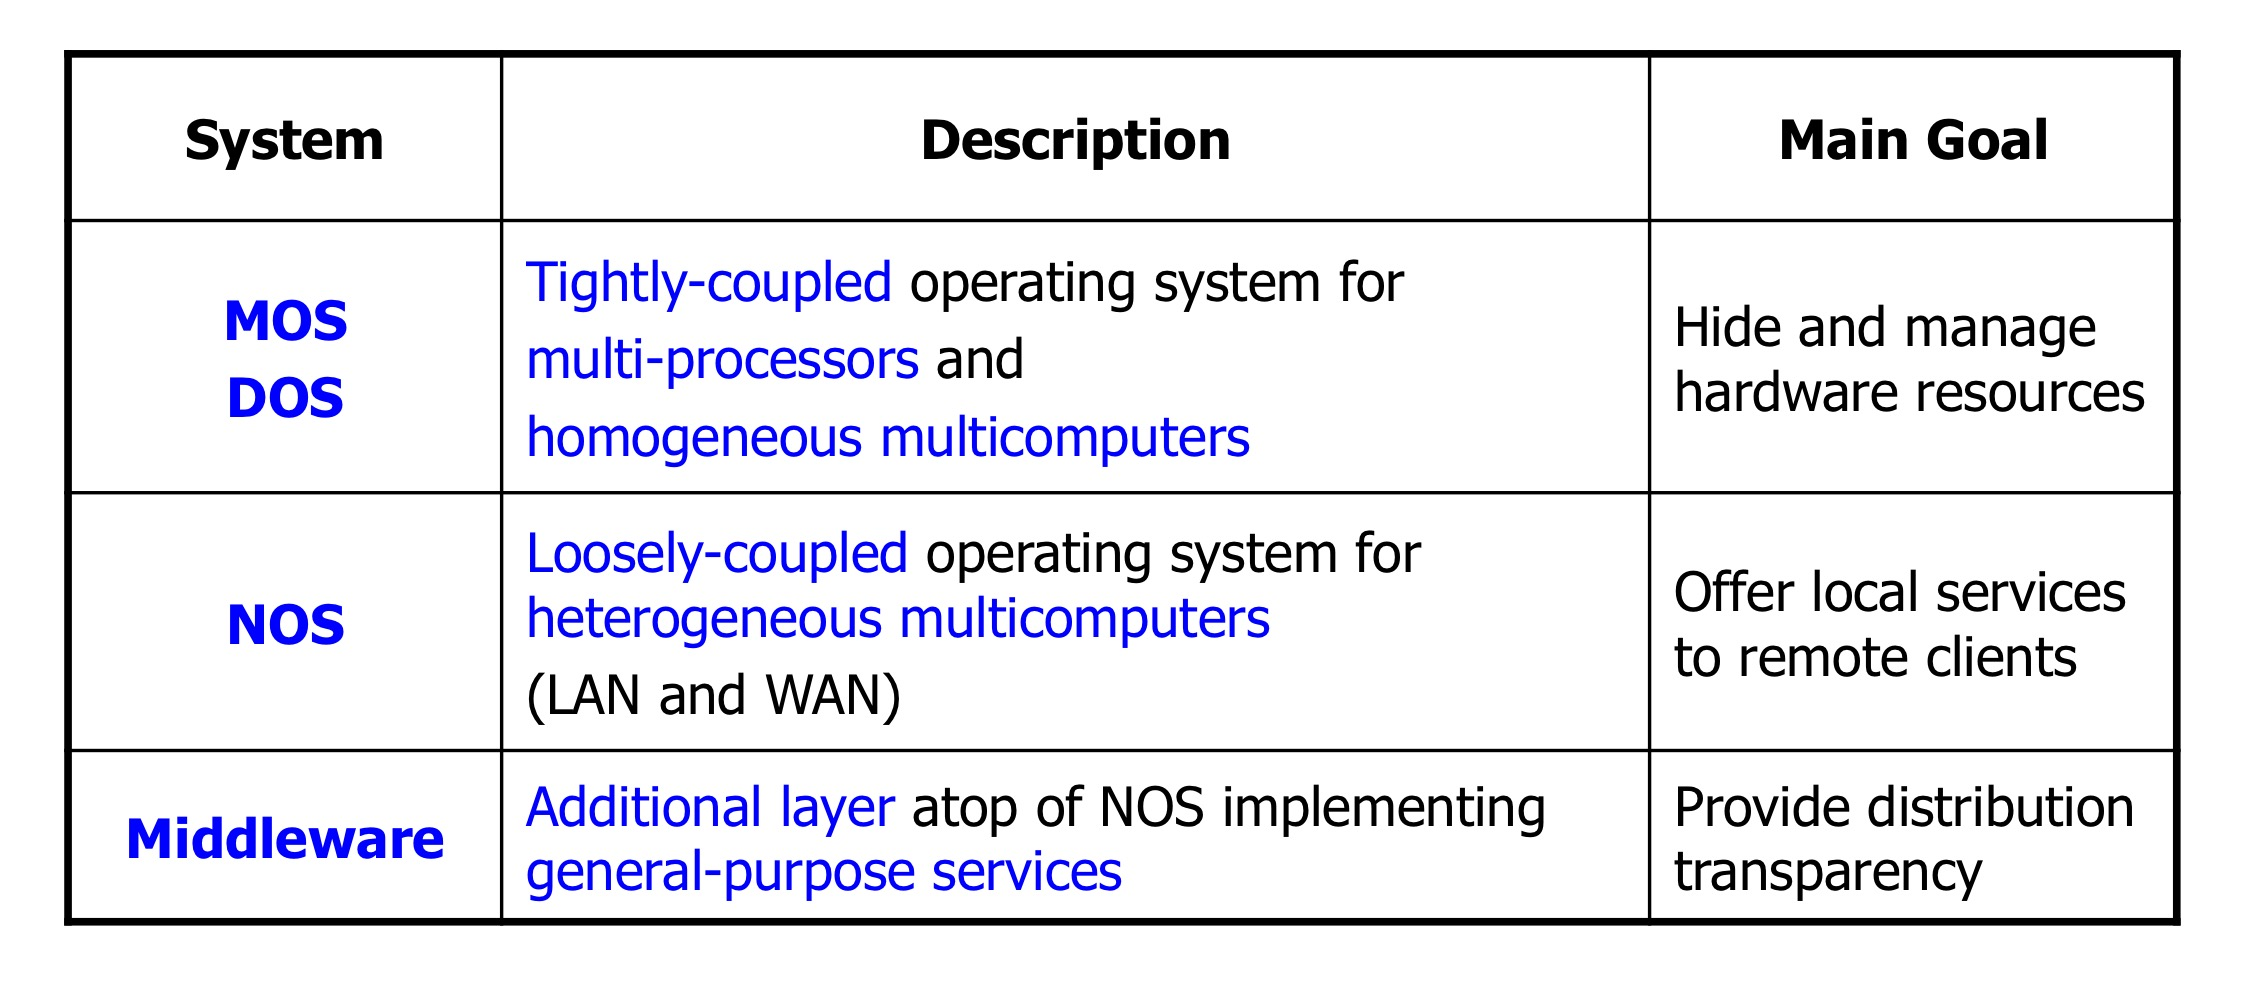
\includegraphics[width=.9\linewidth]{images/distributedSystem/summary1.jpeg}
    \end{figure}
\begin{figure}[!h]
            \centering
            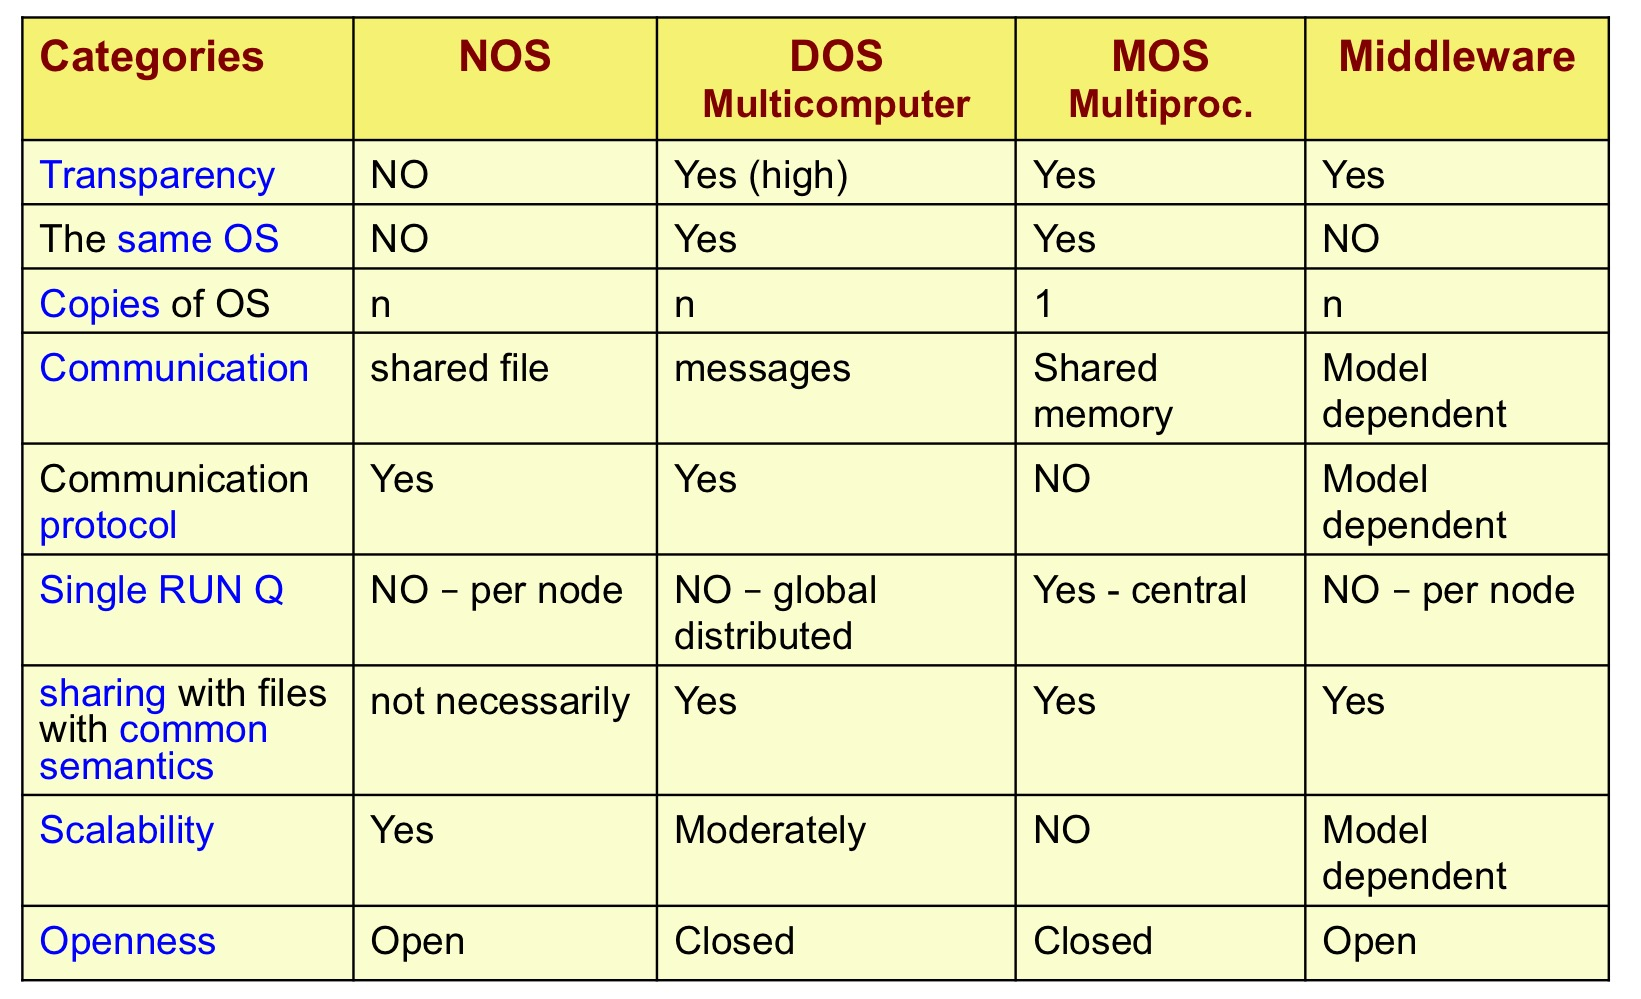
\includegraphics[width=.9\linewidth]{images/distributedSystem/summary2.jpeg}
    \end{figure}